% Status report on the EIC digitisation

\documentclass[a4paper,11pt]{article}
\usepackage[pdftex]{graphicx}
\title{EIC Digitisation status. Version 10}
\date{January 19$^{th}$ 2011}
\author{Philip Brohan}

\begin{document}
\maketitle

This is a summary of the progress of the East-India Company digitisation work: a collection of diagnostics for the new observations produced. I plan to update this document with each new batch of data digitised, and to add additional diagnostics and analyses [suggestions welcome]. About 900 logbooks containing instrumental weather observations were imaged and are being digitised. 784 have been digitised so far. The data so far cover 1788 to 1834 and come from 233 different ships.

\begin{figure}
\begin{center}
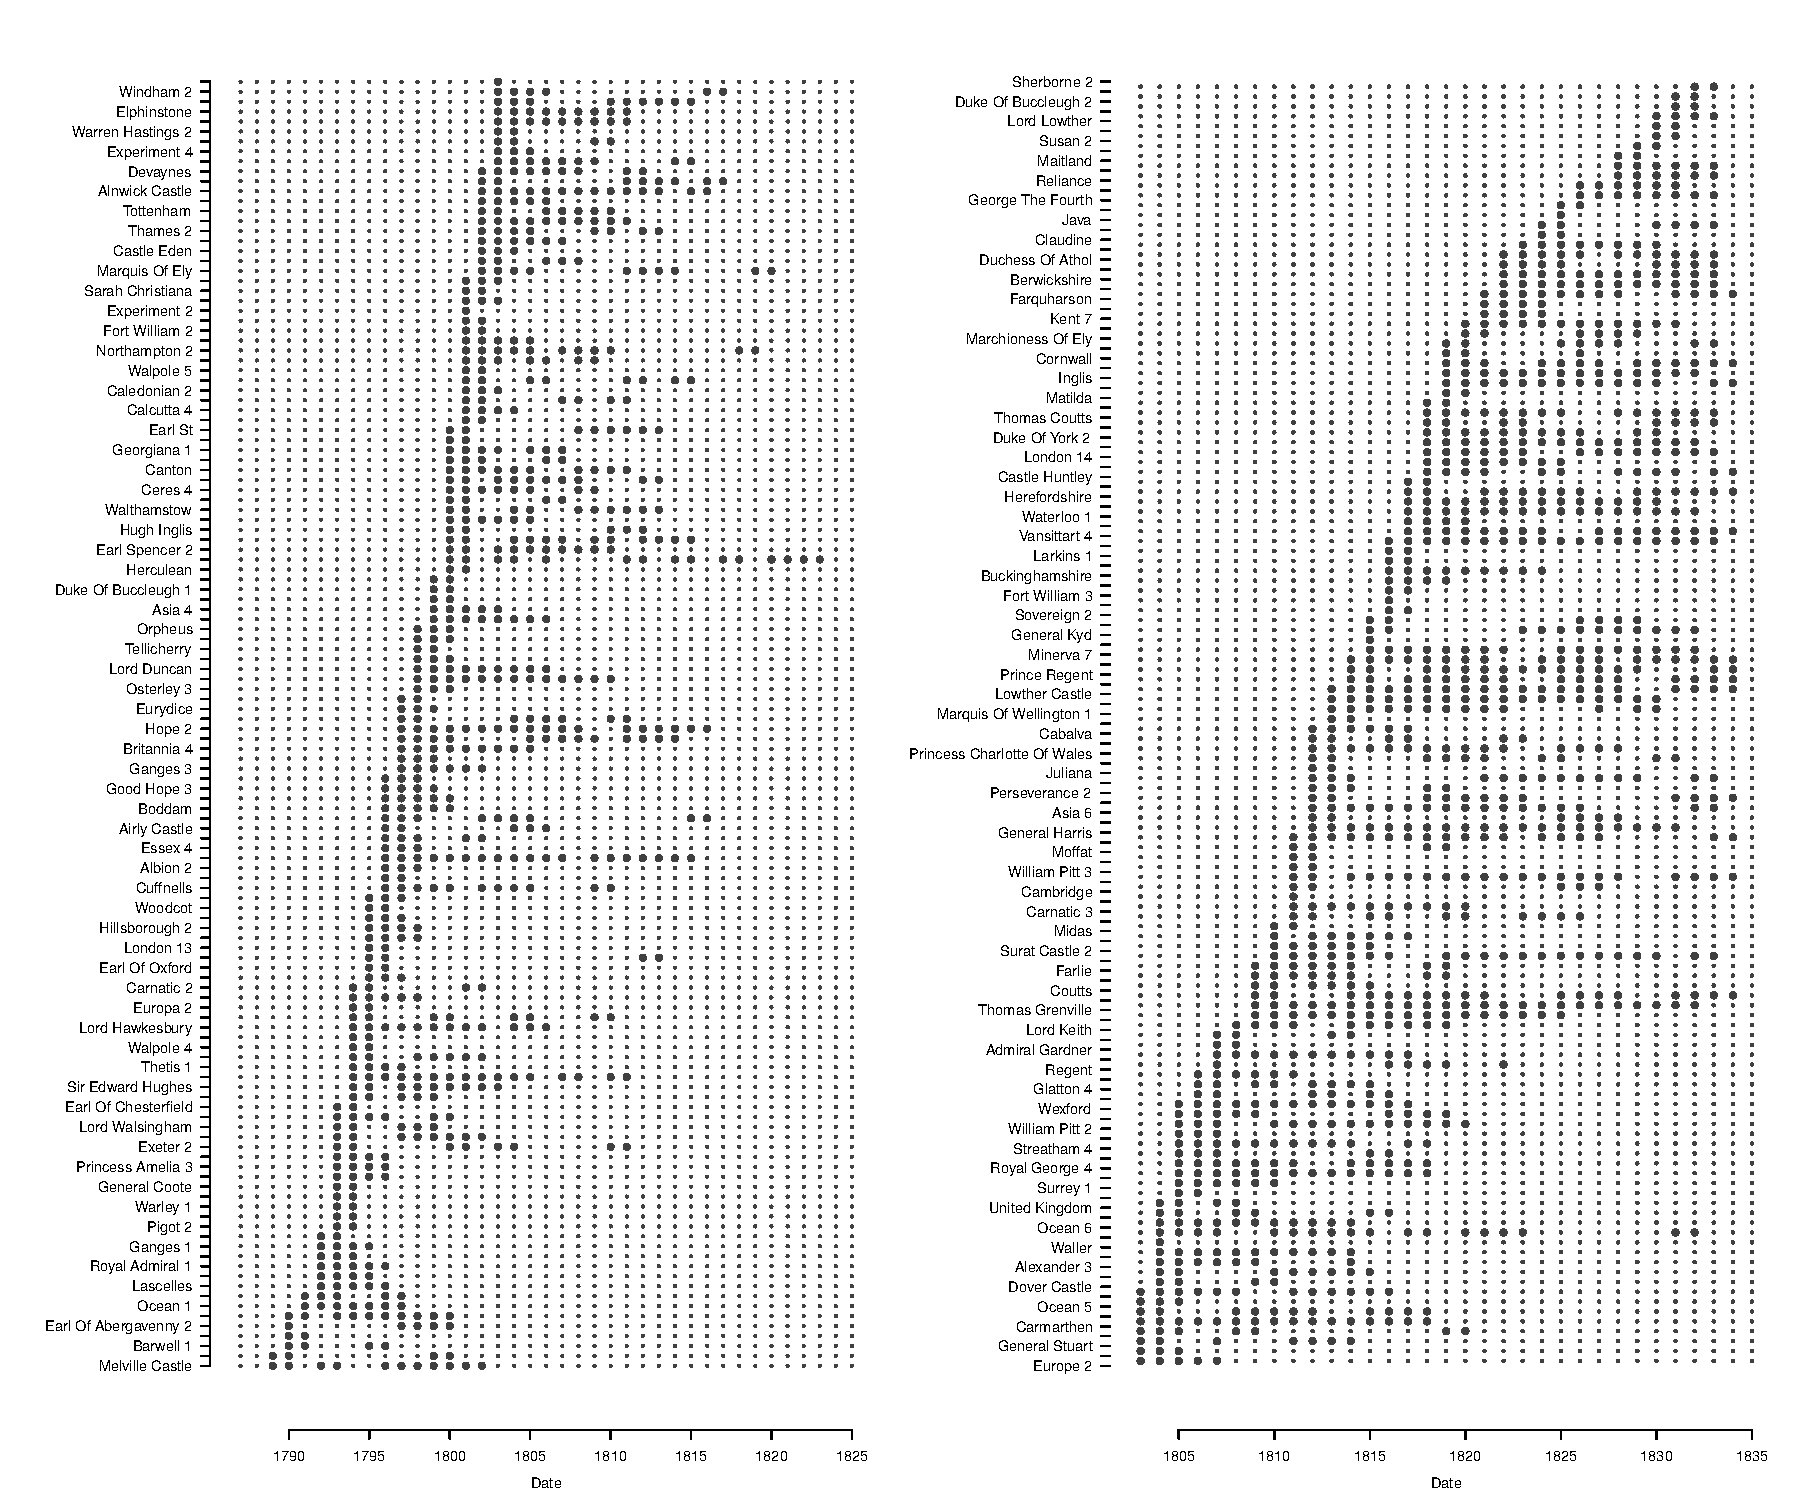
\includegraphics[angle=90, width=1.0\textwidth]{../ships_list/ship_years}
\caption{Period of operation for each ship. One logbook (one trip out and back) usually covers two calendar years.}
\label{ship_years}
\end{center}
\end{figure}

\begin{figure}
\begin{center}
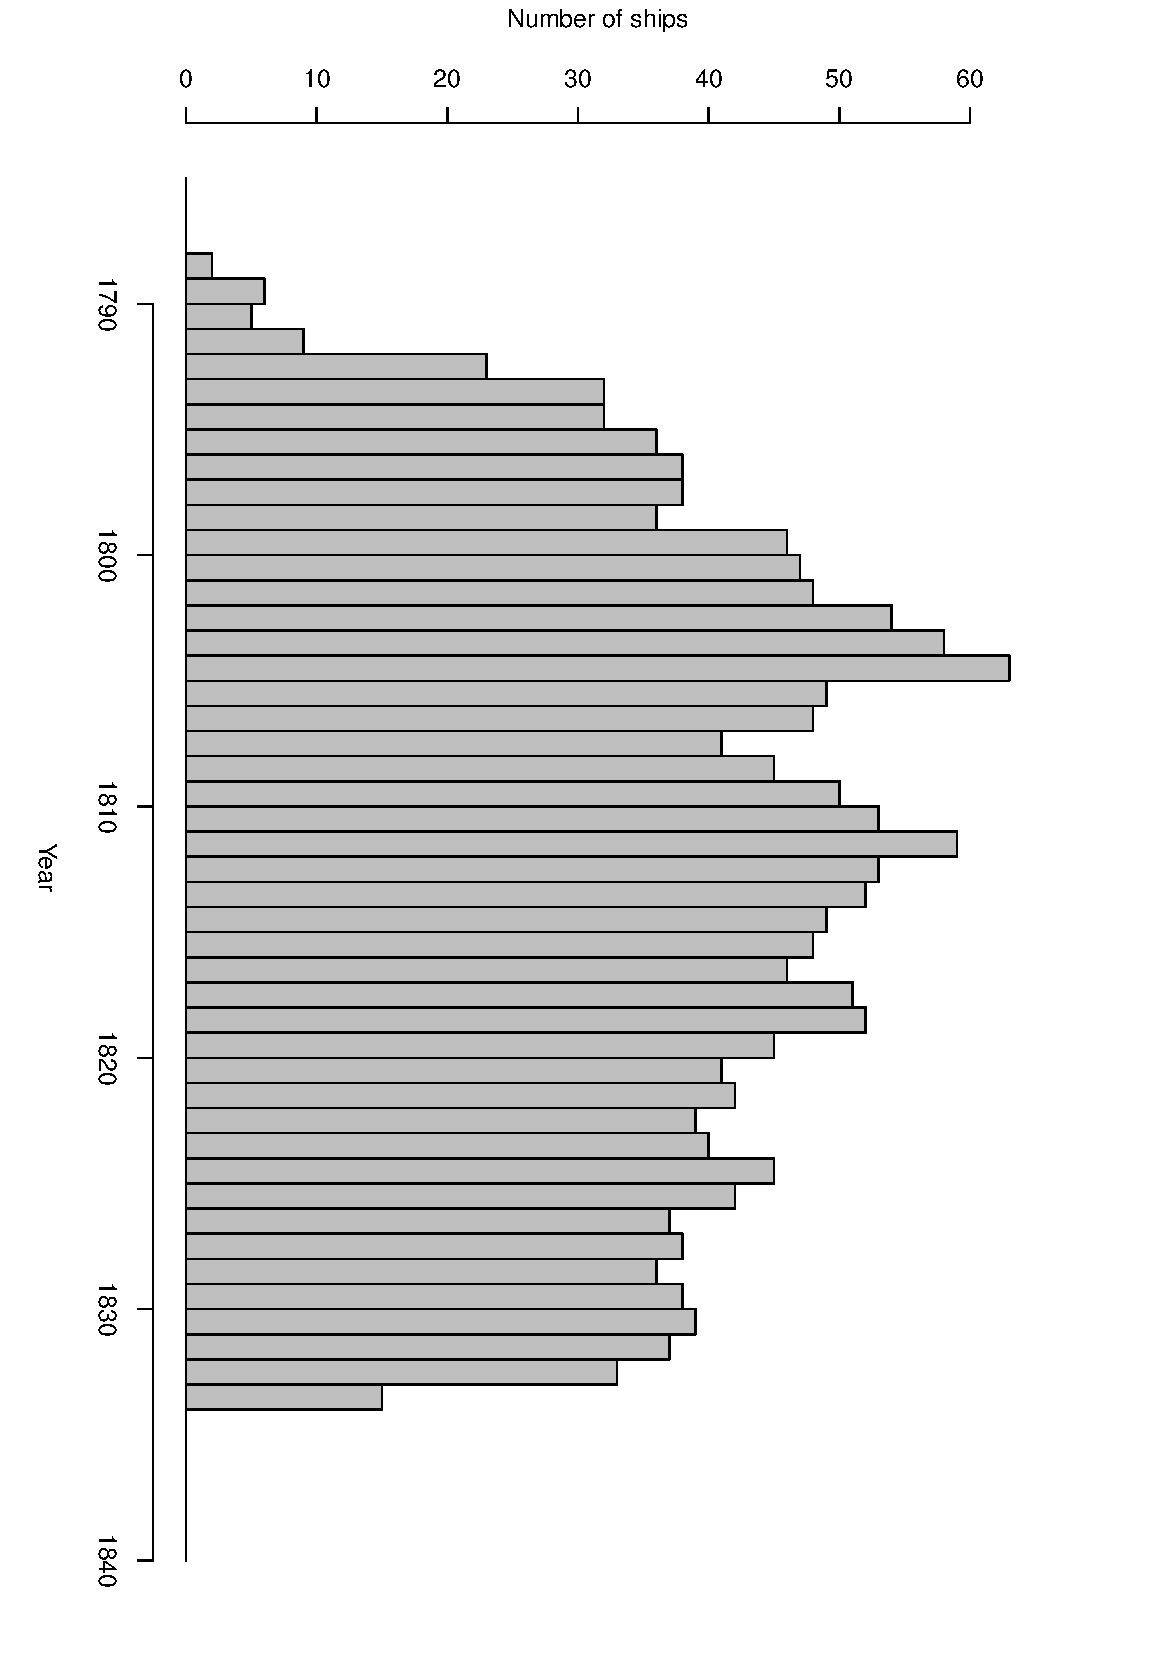
\includegraphics[angle=90, width=1.0\textwidth]{../ships_list/ship_count}
\caption{Number of logs for each year.}
\label{ship_count}
\end{center}
\end{figure}

\begin{figure}
\begin{center}
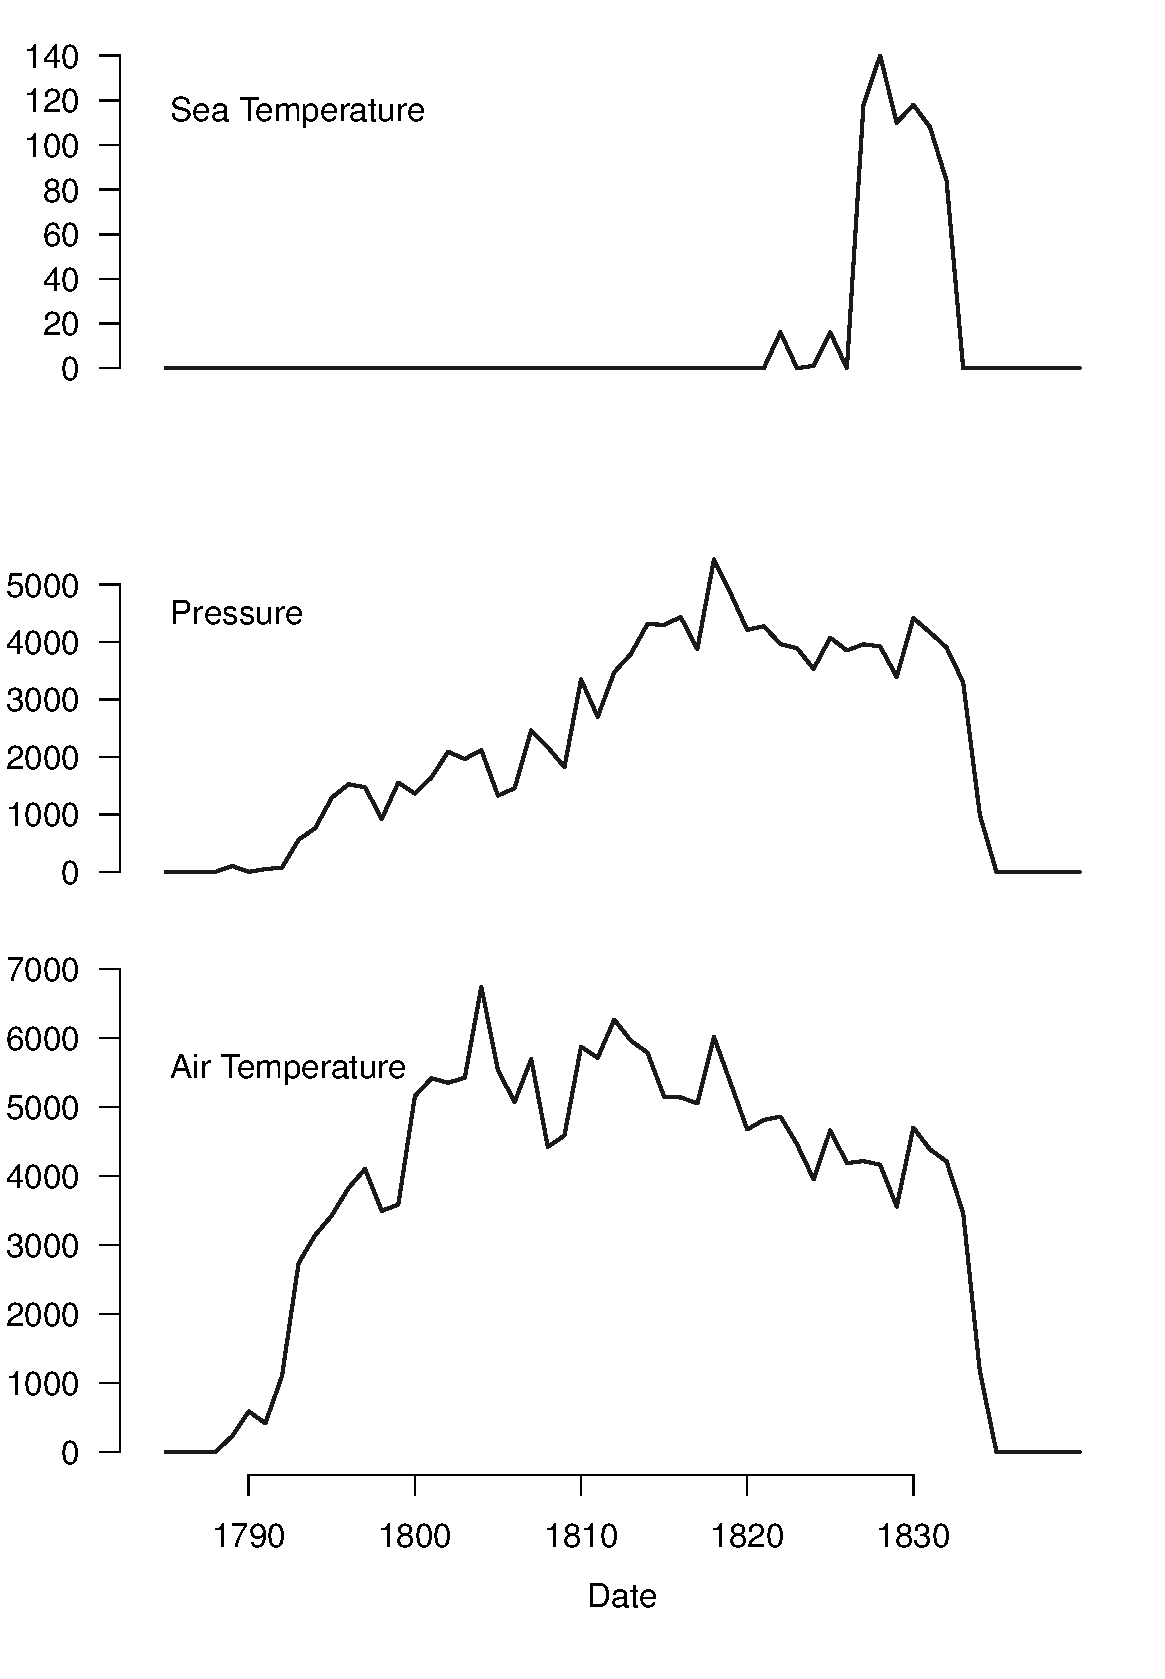
\includegraphics[angle=0, width=1.0\textwidth]{../obs_count/ob_years}
\caption{Number of observations for each year. [Temperatures are more common that pressures in the earlier voyages - I'd have thought pressures would be more important, but perhaps thermometers were cheaper]. Only one log so far has many sea temperature observations (The Thomas Grenville in 1827--8).}
\label{ob_months}
\end{center}
\end{figure}
\begin{figure}
\begin{center}
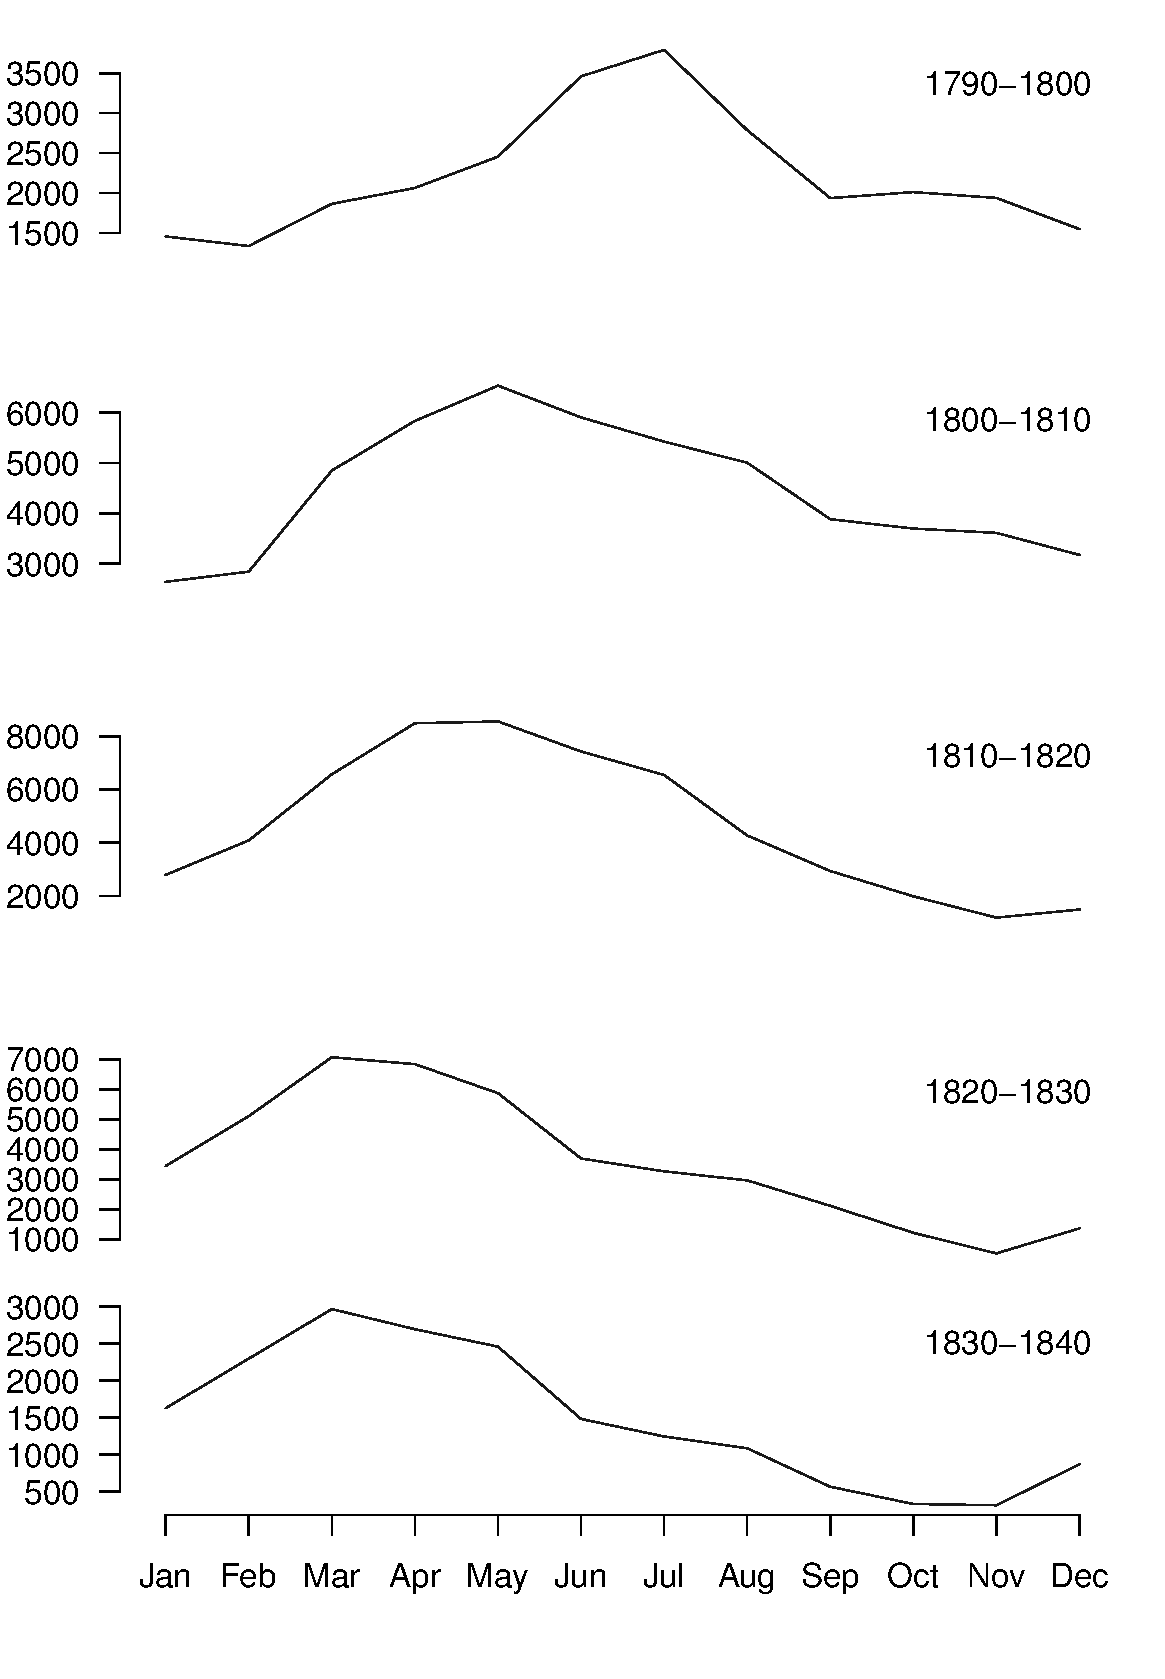
\includegraphics[angle=0, width=1.0\textwidth]{../obs_count/ob_seasonal}
\caption{Seasonal cycle in the number of air temperature observations - averages for each decade. [Clear change in seasonality over the period - why?]}
\label{ob_seasonal}
\end{center}
\end{figure}

\begin{figure}
\begin{center}
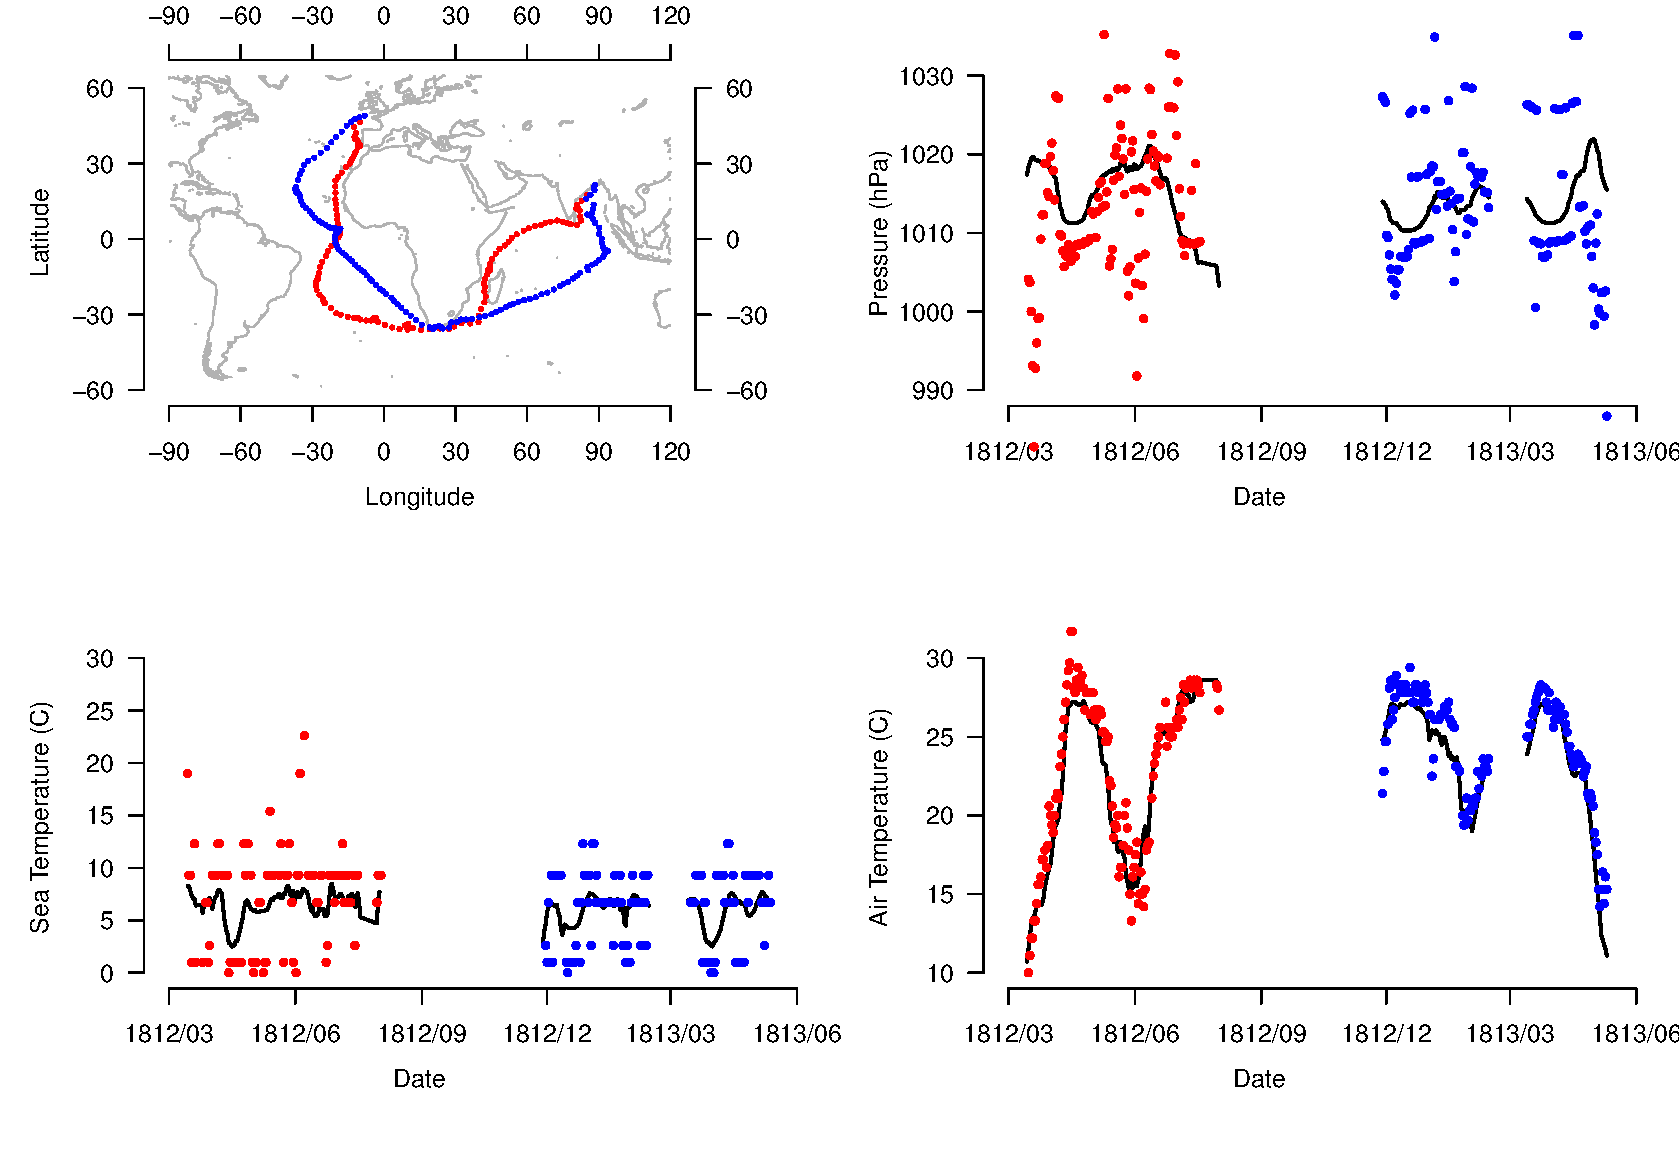
\includegraphics[angle=0, width=1.0\textwidth]{../individual_logs/Astell_1812-13/Astell}
\caption{A sample voyage: Observations from the outward (red) and return (blue) voyages of the {\it Astell} in 1812--13. Coloured points are the daily (noon) positions and weather observations recorded in the logbook, black lines show the expected values from 1961--90 climatologies for a ship following the same route at the same time of year. [AT expected high as it's a noon observation, big scatter in the pressure not surprising, wind speeds look promising, though beaufort quantisation makes them hard to compare].}
\label{astell}
\end{center}
\end{figure}

\begin{figure}
\begin{center}
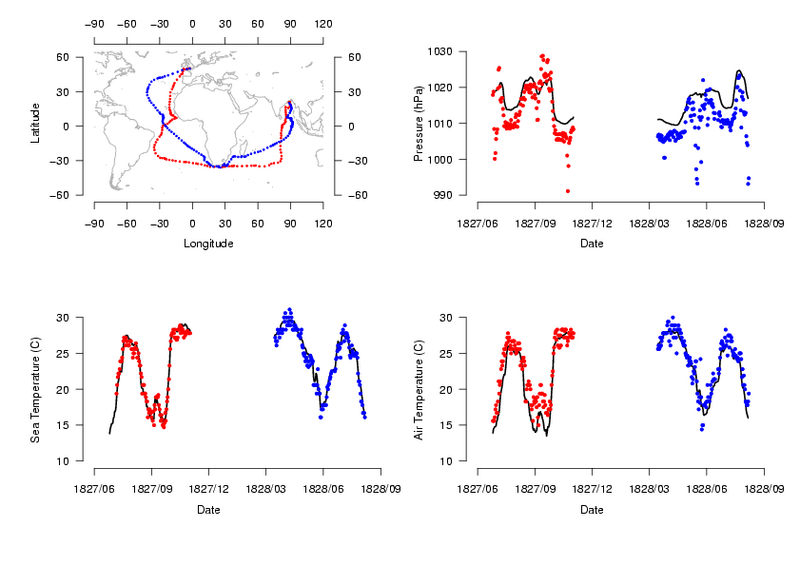
\includegraphics[angle=0, width=1.0\textwidth]{../individual_logs/Thomas_Grenville_1827-8/Thomas_Grenville}
\caption{A sample voyage: Observations from the outward (red) and return (blue) voyages of the {\it Thomas Grenville} in 1827--8. Coloured points are the daily (noon) positions and weather observations recorded in the logbook, black lines show the expected values from 1961--90 climatologies for a ship following the same route at the same time of year. [AT expected high as it's a noon observation, why is the pressure low?]. This is the only log (so far) with many sea-temperature data. [Quite different choice of route from the Astell's - is this because they started in June rather than March?]}
\label{thomas_grenville}
\end{center}
\end{figure}

\begin{figure}
\begin{center}
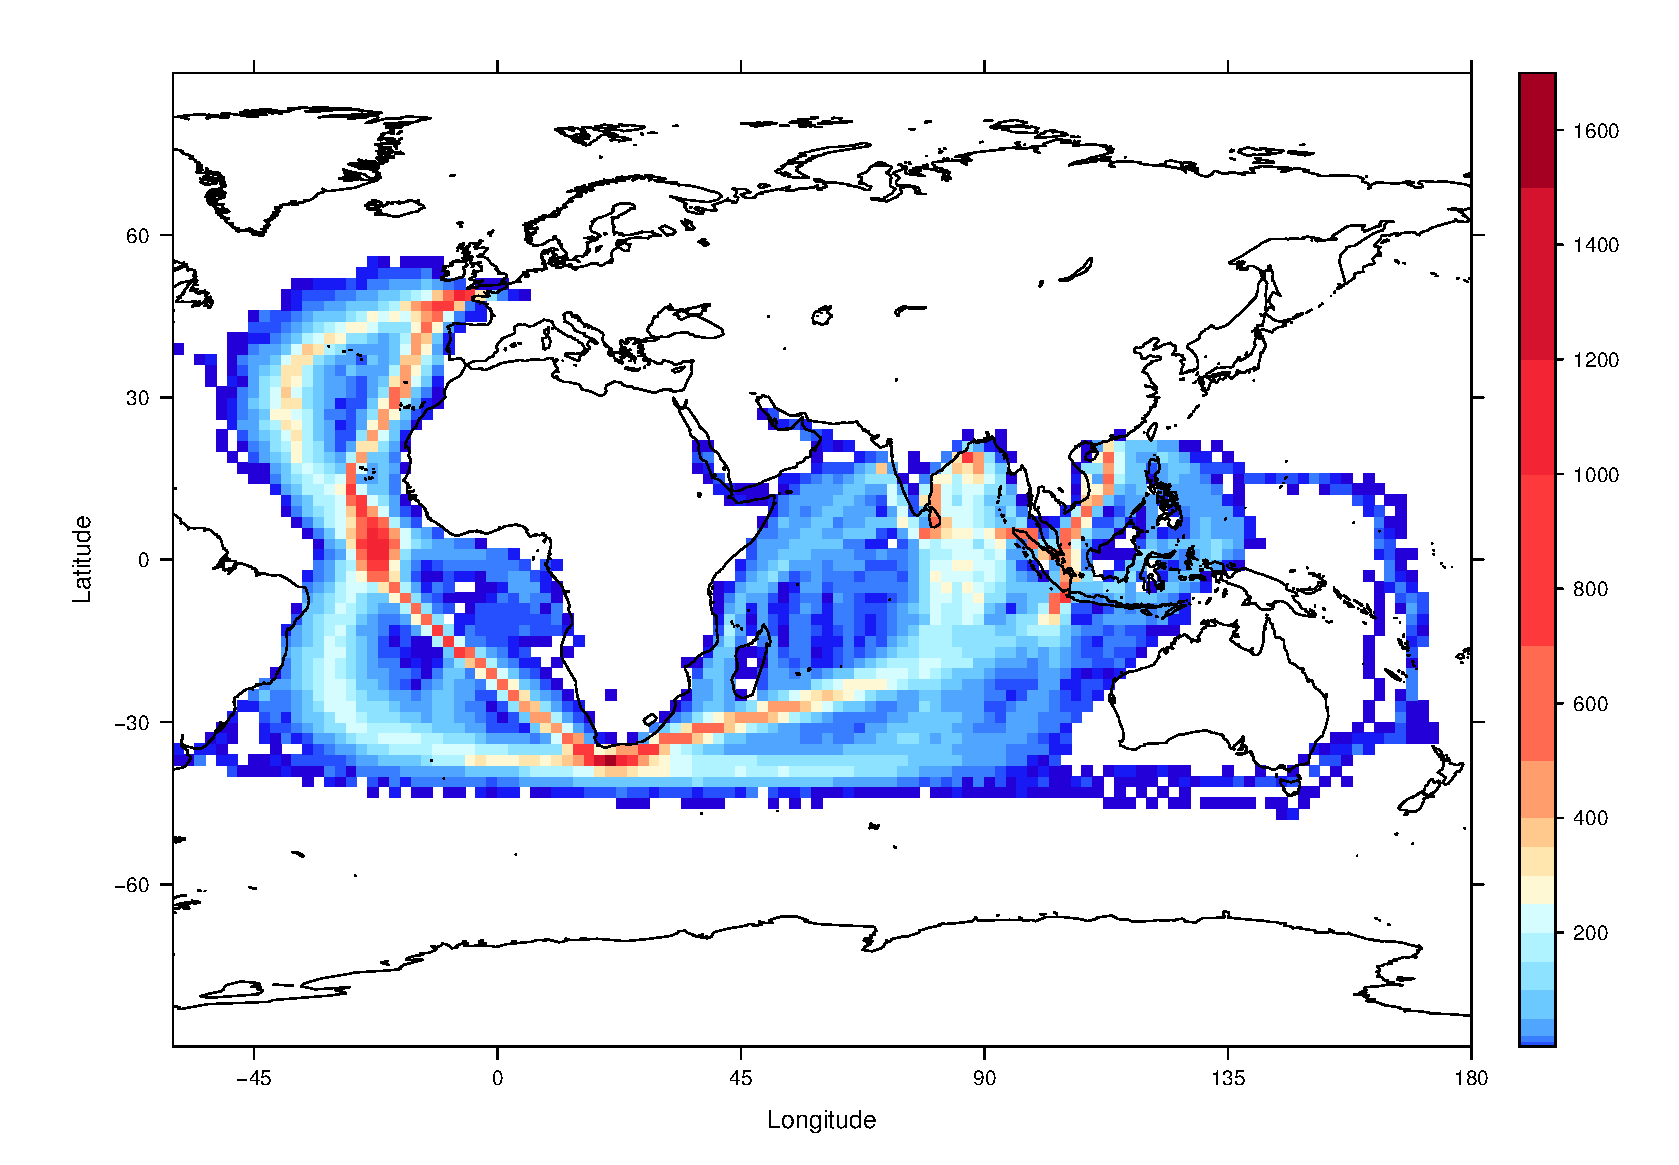
\includegraphics[angle=0, width=1.0\textwidth]{../coverage_map/coverage}
\caption{Total number of observations in each $2^\circ$ by $2^\circ$ square. [Still some uncorrected positional errors - and the odd maverick: the voyage going round Australia is a convoy in 1804/5 - sent that way to avoid a French squadron in the Indian Ocean. The best route out and back is obviously prety well agreed on, except in the Indian Ocean on the way out, where the choices made by the Astell (figure \ref{astell} and Thomas Grenville (figure \ref{thomas_grenville}) both have adherents.]}
\label{coverage}
\end{center}
\end{figure}

\clearpage

\begin{figure}
\begin{center}
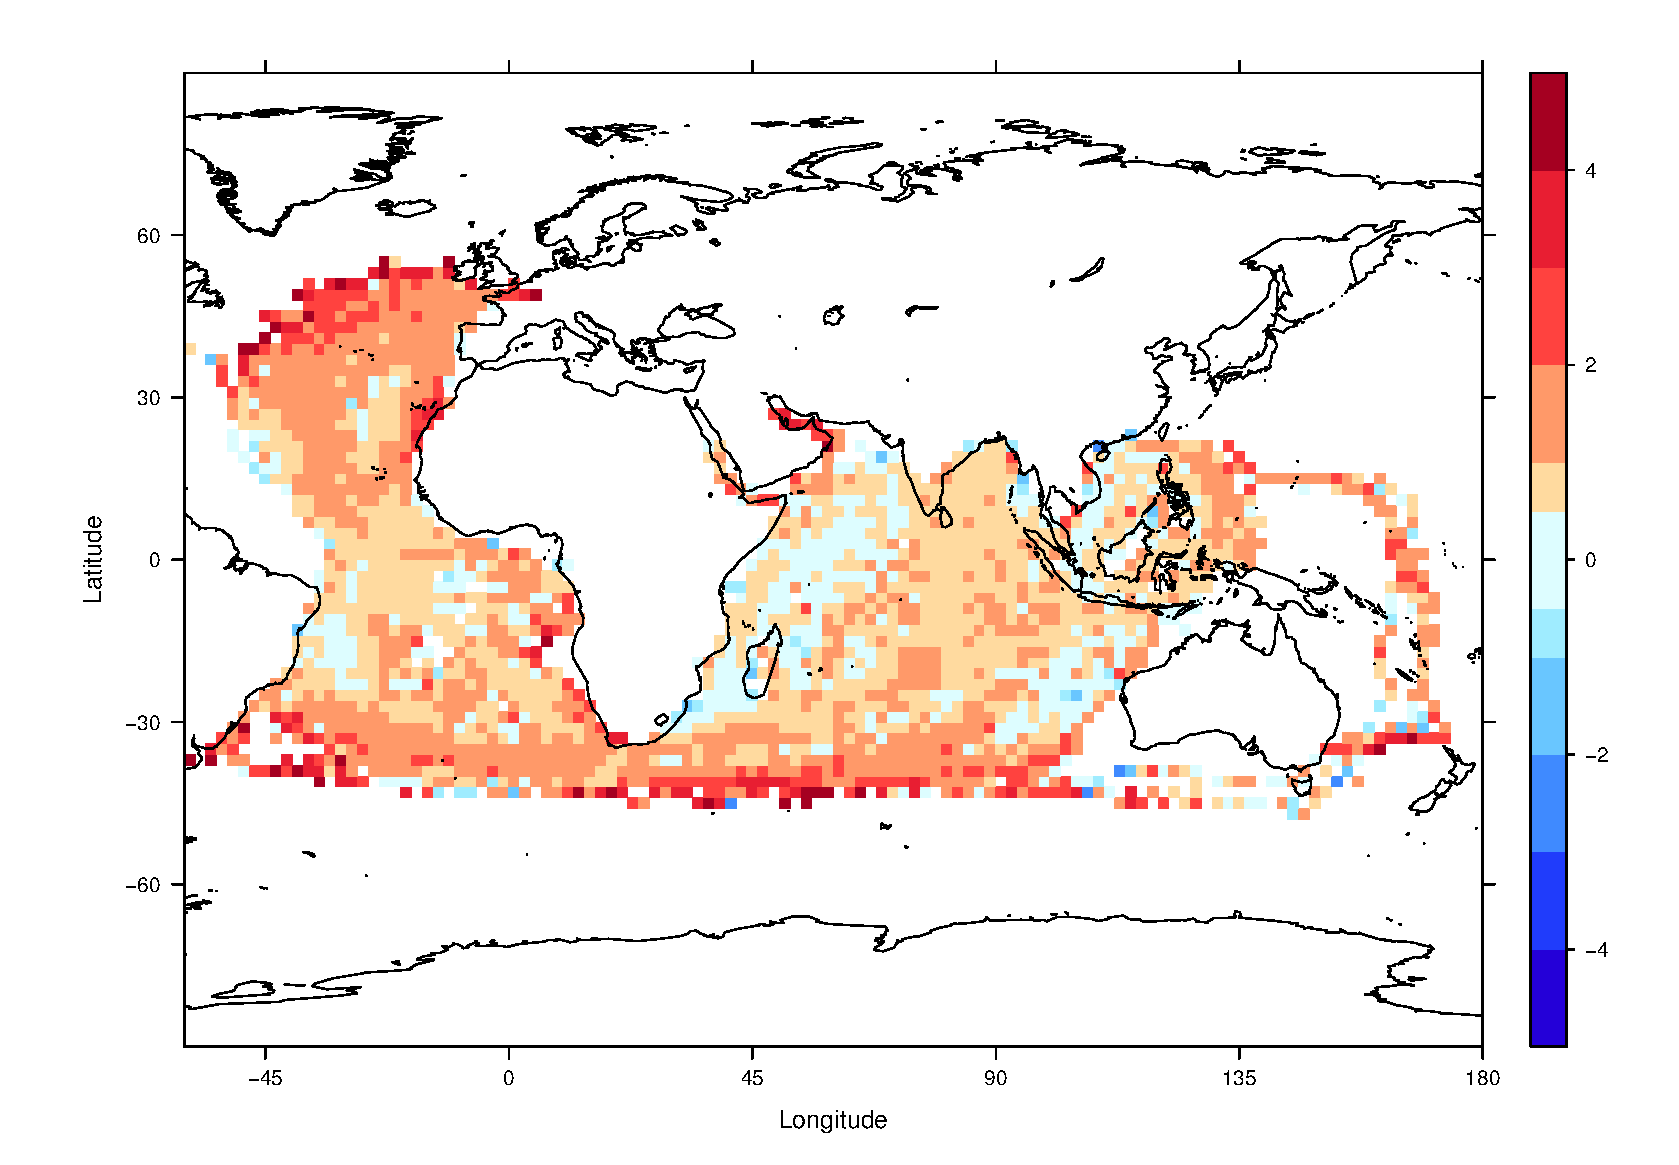
\includegraphics[angle=0, width=1.0\textwidth]{../anomaly_map/at_anomaly}
\caption{Truncated mean air-temperature anomaly (observation minus HadNAT2 climatology) in each $2^\circ$ by $2^\circ$ square. [A positive AT anomaly was expected because of ship heating and inadequate thermometer screens].}
\label{at_anomaly}
\end{center}
\end{figure}

\begin{figure}
\begin{center}
\includegraphics[angle=0, width=1.0\textwidth]{../anomaly_ts/at_anom_ts}
\caption{Time-series of air-temperature anomalies (observation minus HadNAT2 climatology). Each point is one measurement, the different colours are different ships (though there are more ships than available colours). [Not a very useful plot for showing time-variation, but does show up the seasonality of the data, and the large variation in scatter between the different ships.] }
\label{at_anom_ts}
\end{center}
\end{figure}

\begin{figure}
\begin{center}
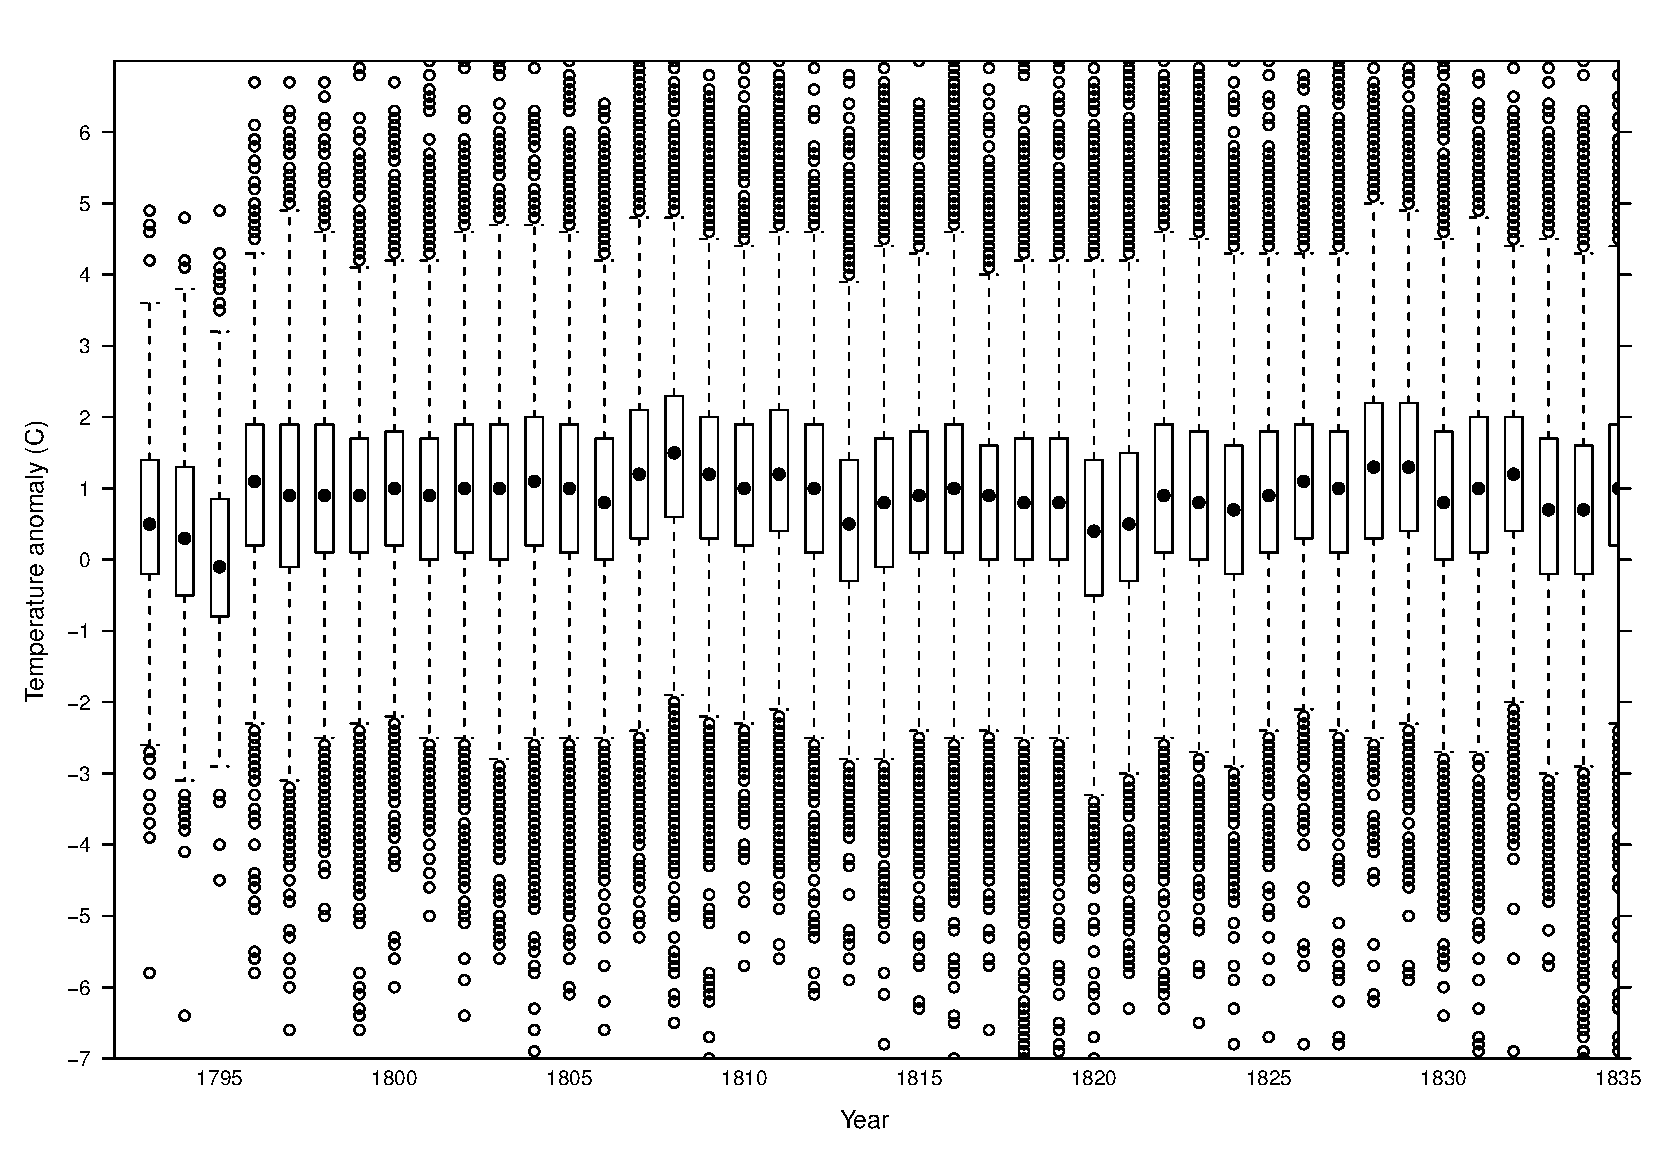
\includegraphics[angle=0, width=1.0\textwidth]{../anomaly_ts/at_anom_bwplot}
\caption{Time-series of air-temperature anomalies (observation minus HadNAT2 climatology). Box-and-whisker plot with the anomalies aggregated by calendar year. [No sign of the Tambora eruption (or the 1809 eruption) - though this is not the most powerful method for looking at small changes in the mean].}
\label{at_anom_bwplot}
\end{center}
\end{figure}

\begin{figure}
\begin{center}
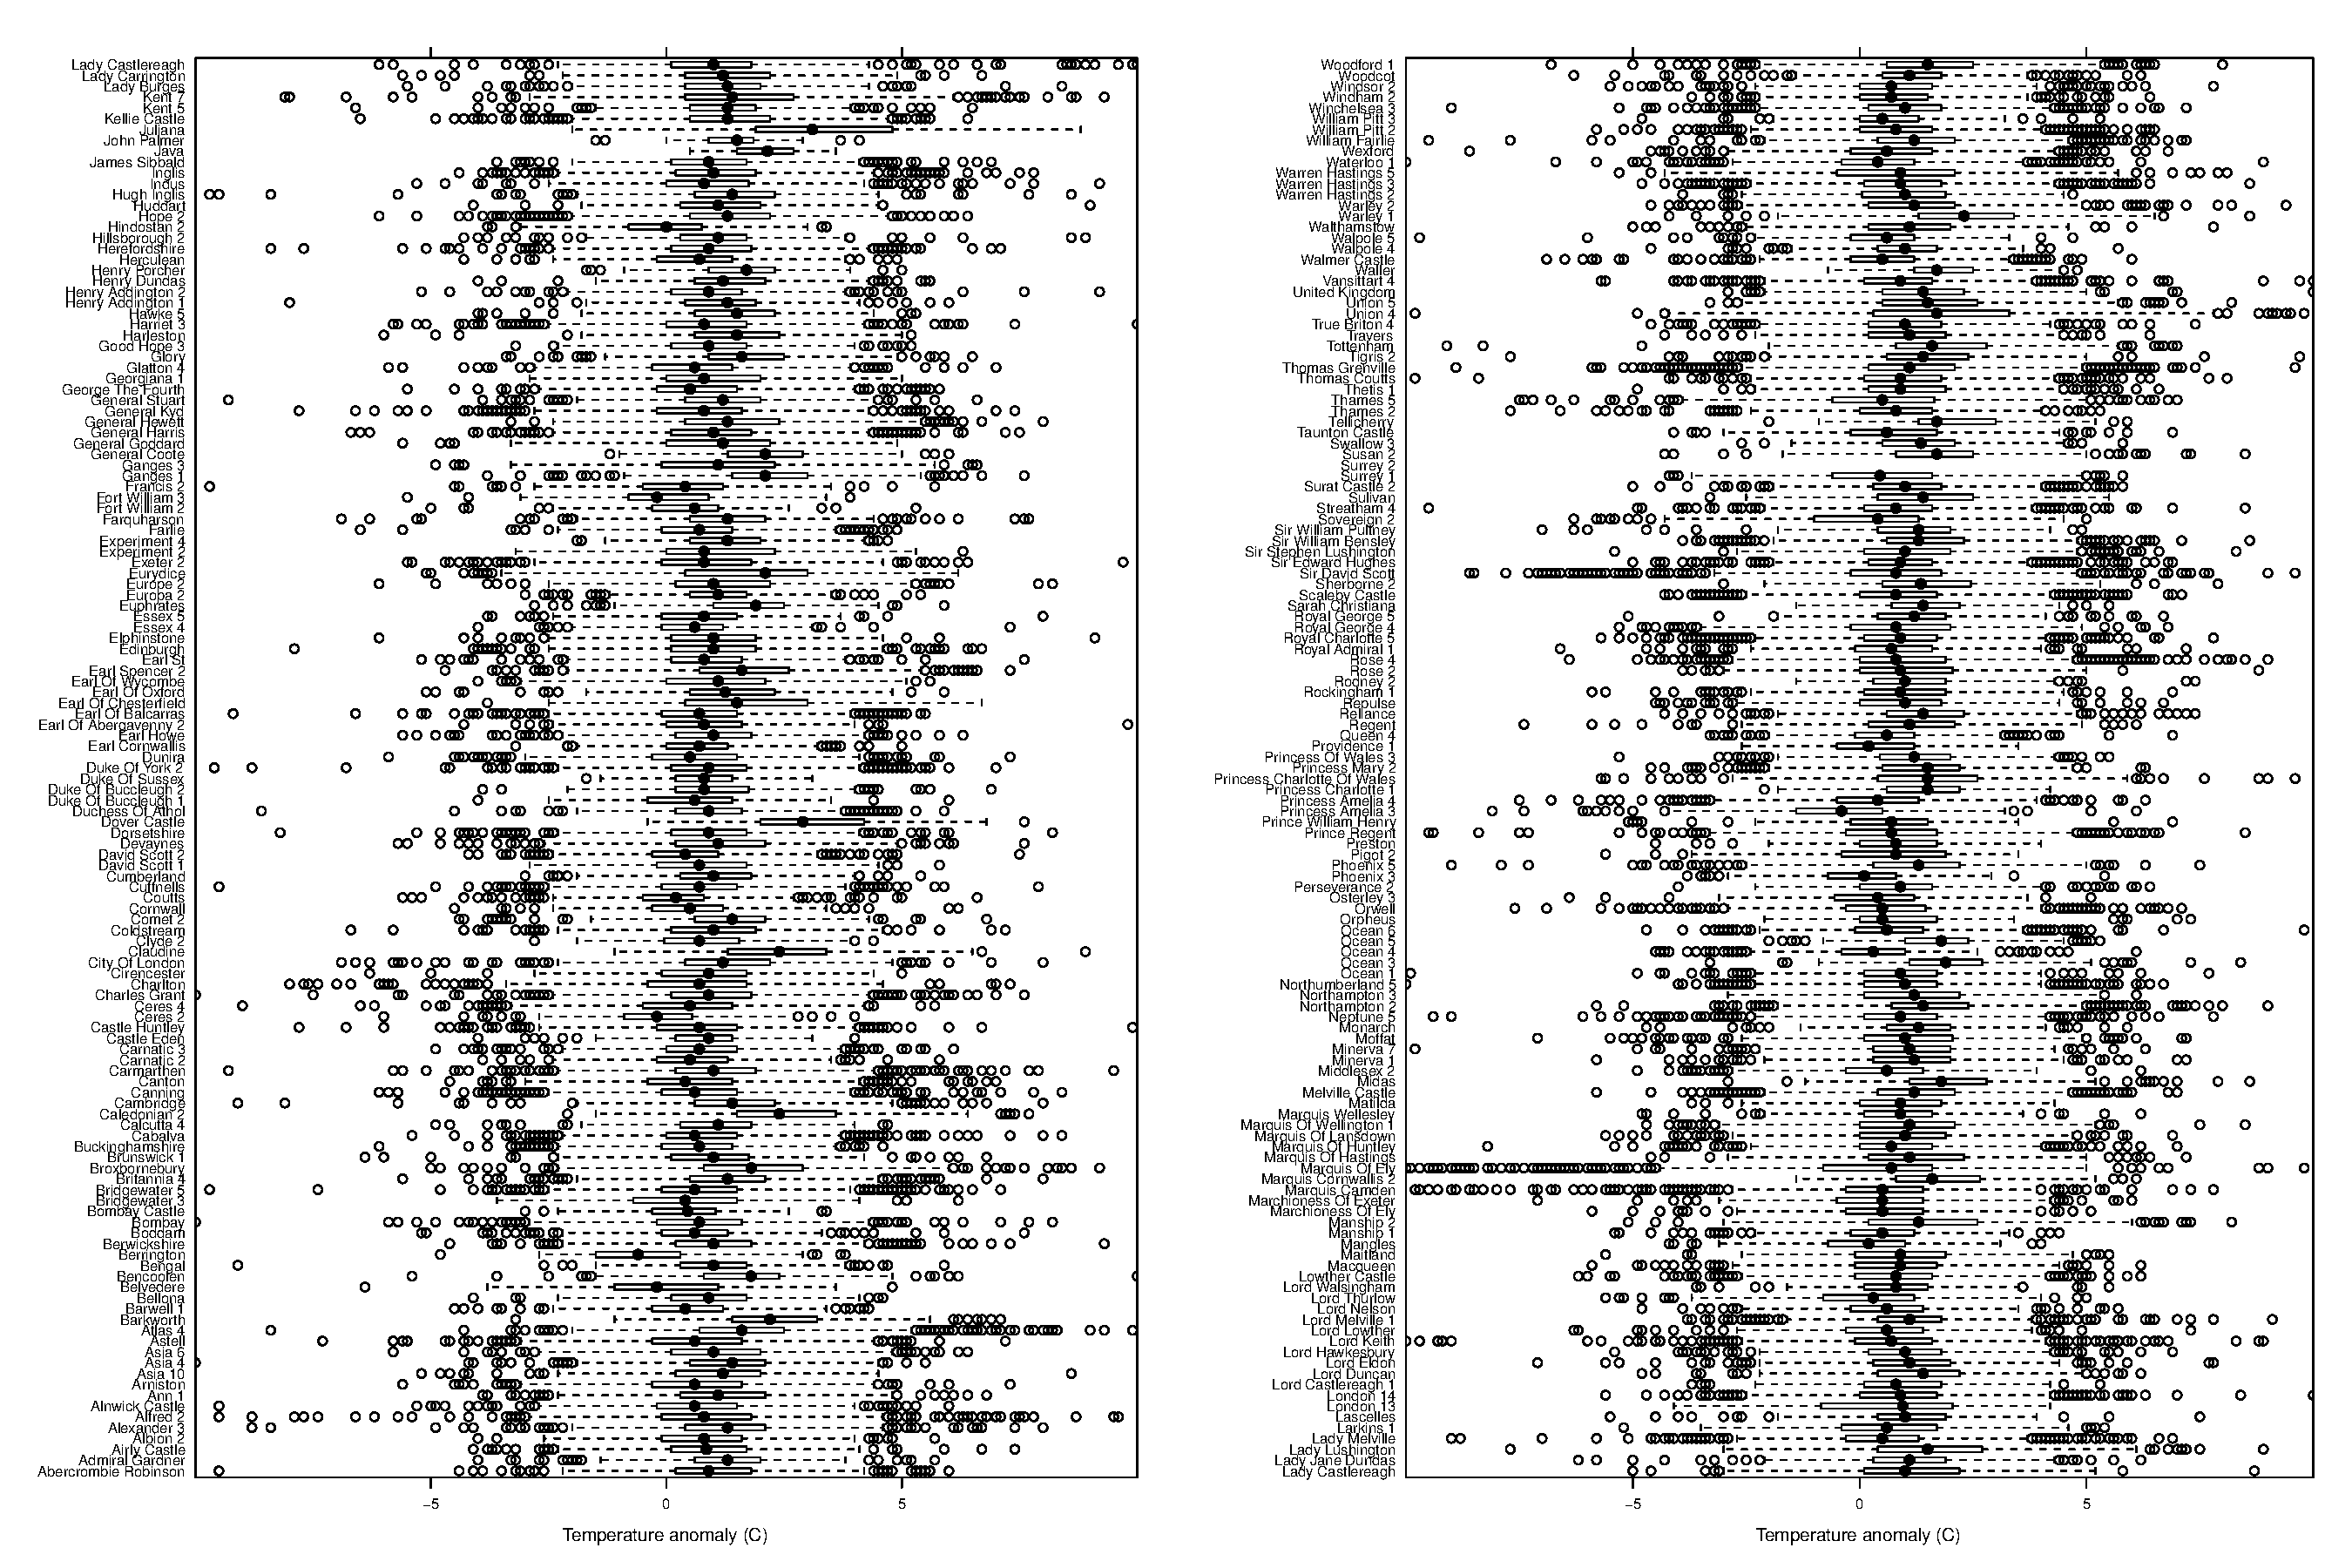
\includegraphics[angle=90, width=1.0\textwidth]{../anomaly_ts/at_anom_bwplot_byShip}
\caption{Between-ship variability of air-temperature anomalies (observation minus HadNAT2 climatology). Box-and-whisker plot with the anomalies aggregated by ship.}
\label{at_anom_bwplot_byShip}
\end{center}
\end{figure}

\clearpage

\begin{figure}
\begin{center}
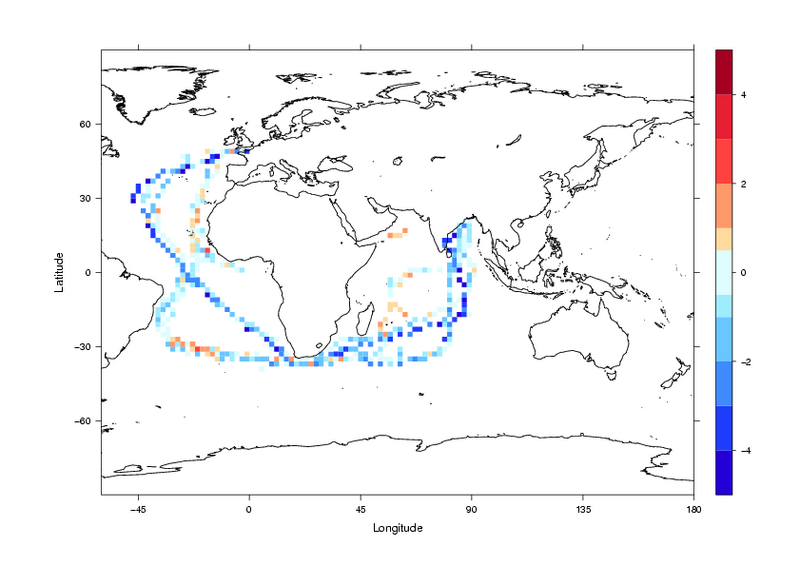
\includegraphics[angle=0, width=1.0\textwidth]{../anomaly_map/sst_anomaly}
\caption{Truncated mean sea-temperature anomaly (observation minus HadSST2 climatology) in each $2^\circ$ by $2^\circ$ square. [Only really data from one log - can't say much.]}
\label{sst_anomaly}
\end{center}
\end{figure}

\begin{figure}
\begin{center}
\includegraphics[angle=0, width=1.0\textwidth]{../anomaly_ts/sst_anom_ts}
\caption{Time-series of sea-temperature anomalies (observation minus HadSST2 climatology). Each point is one measurement, the different colours are different ships (though there are more ships than available colours). [Much less scatter than AT, and less bias too - more data please.] }
\label{sst_anom_ts}
\end{center}
\end{figure}

\clearpage

\begin{figure}
\begin{center}
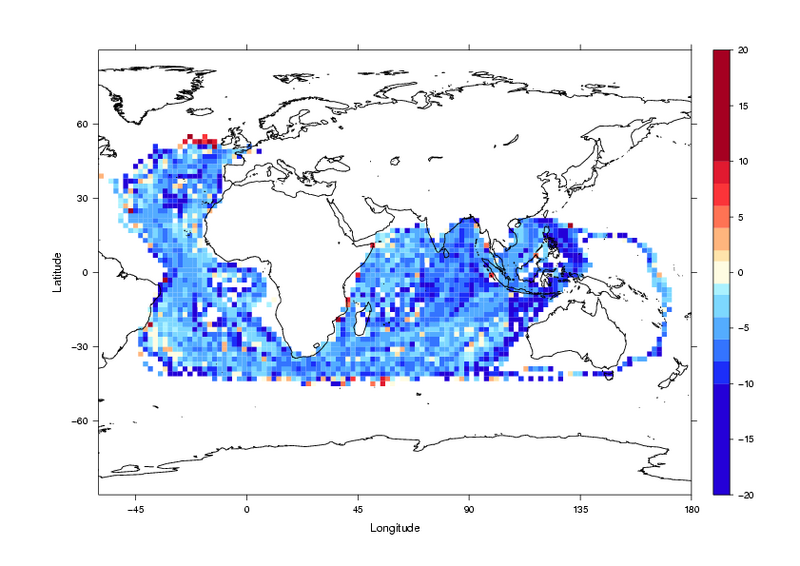
\includegraphics[angle=0, width=1.0\textwidth]{../anomaly_map/pre_anomaly}
\caption{Mean pressure anomaly (observation minus HadSLP2 climatology) in each $2^\circ$ by $2^\circ$ square. [No obvious spatial pattern, but consistently low - why?]}
\label{pressure_anomaly}
\end{center}
\end{figure}

\begin{figure}
\begin{center}
\includegraphics[angle=0, width=1.0\textwidth]{../anomaly_ts/pre_anom_ts}
\caption{Time-series of barometer pressure anomalies (observation minus HadSLP2 climatology). Each point is one measurement, the different colours are different ships (though there are more ships than available colours). [What should this tell us? Noticeable inter-ship biases.] }
\label{pre_anom_ts}
\end{center}
\end{figure}

\begin{figure}
\begin{center}
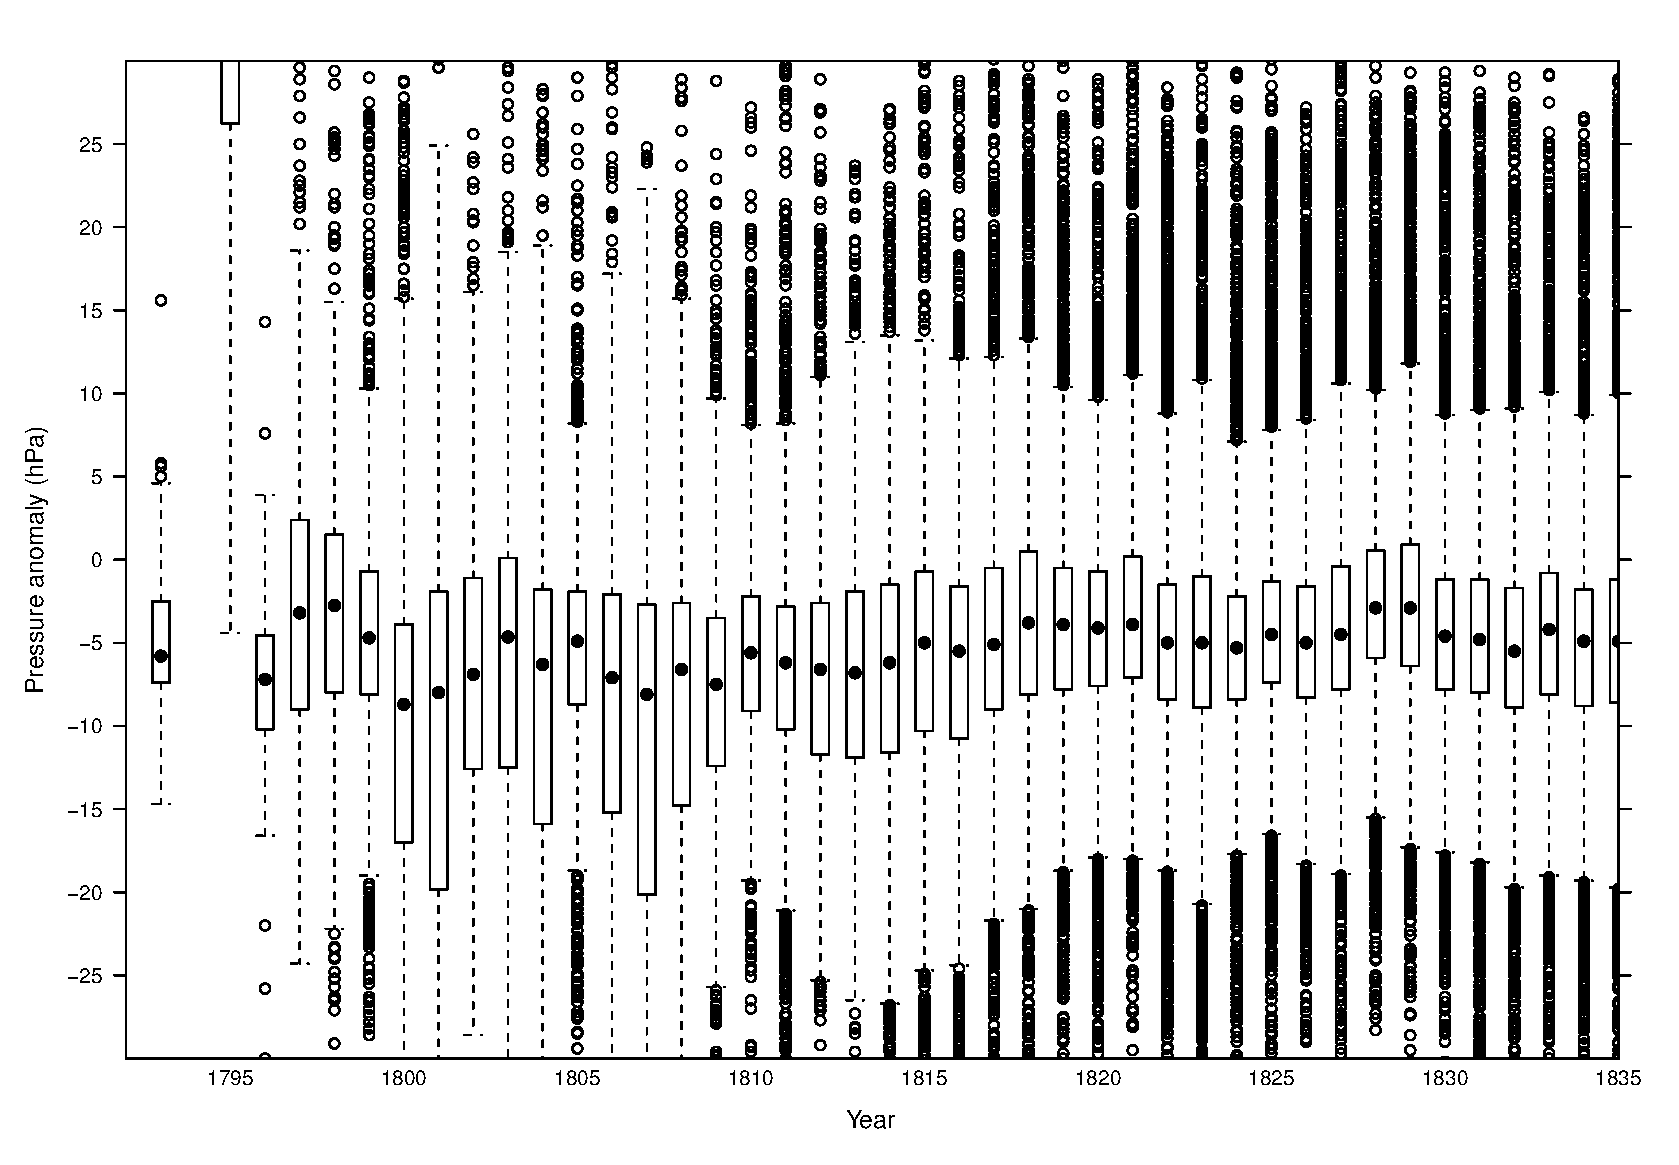
\includegraphics[angle=0, width=1.0\textwidth]{../anomaly_ts/pre_anom_bwplot}
\caption{Time-series of barometer pressure anomalies (observation minus HadSLP2 climatology). Box-and-whisker plot with the anomalies aggregated by calendar year. [The variability is probably mostly inter-ship effects - see next figure.]}
\label{pre_anom_bwplot}
\end{center}
\end{figure}

\begin{figure}
\begin{center}
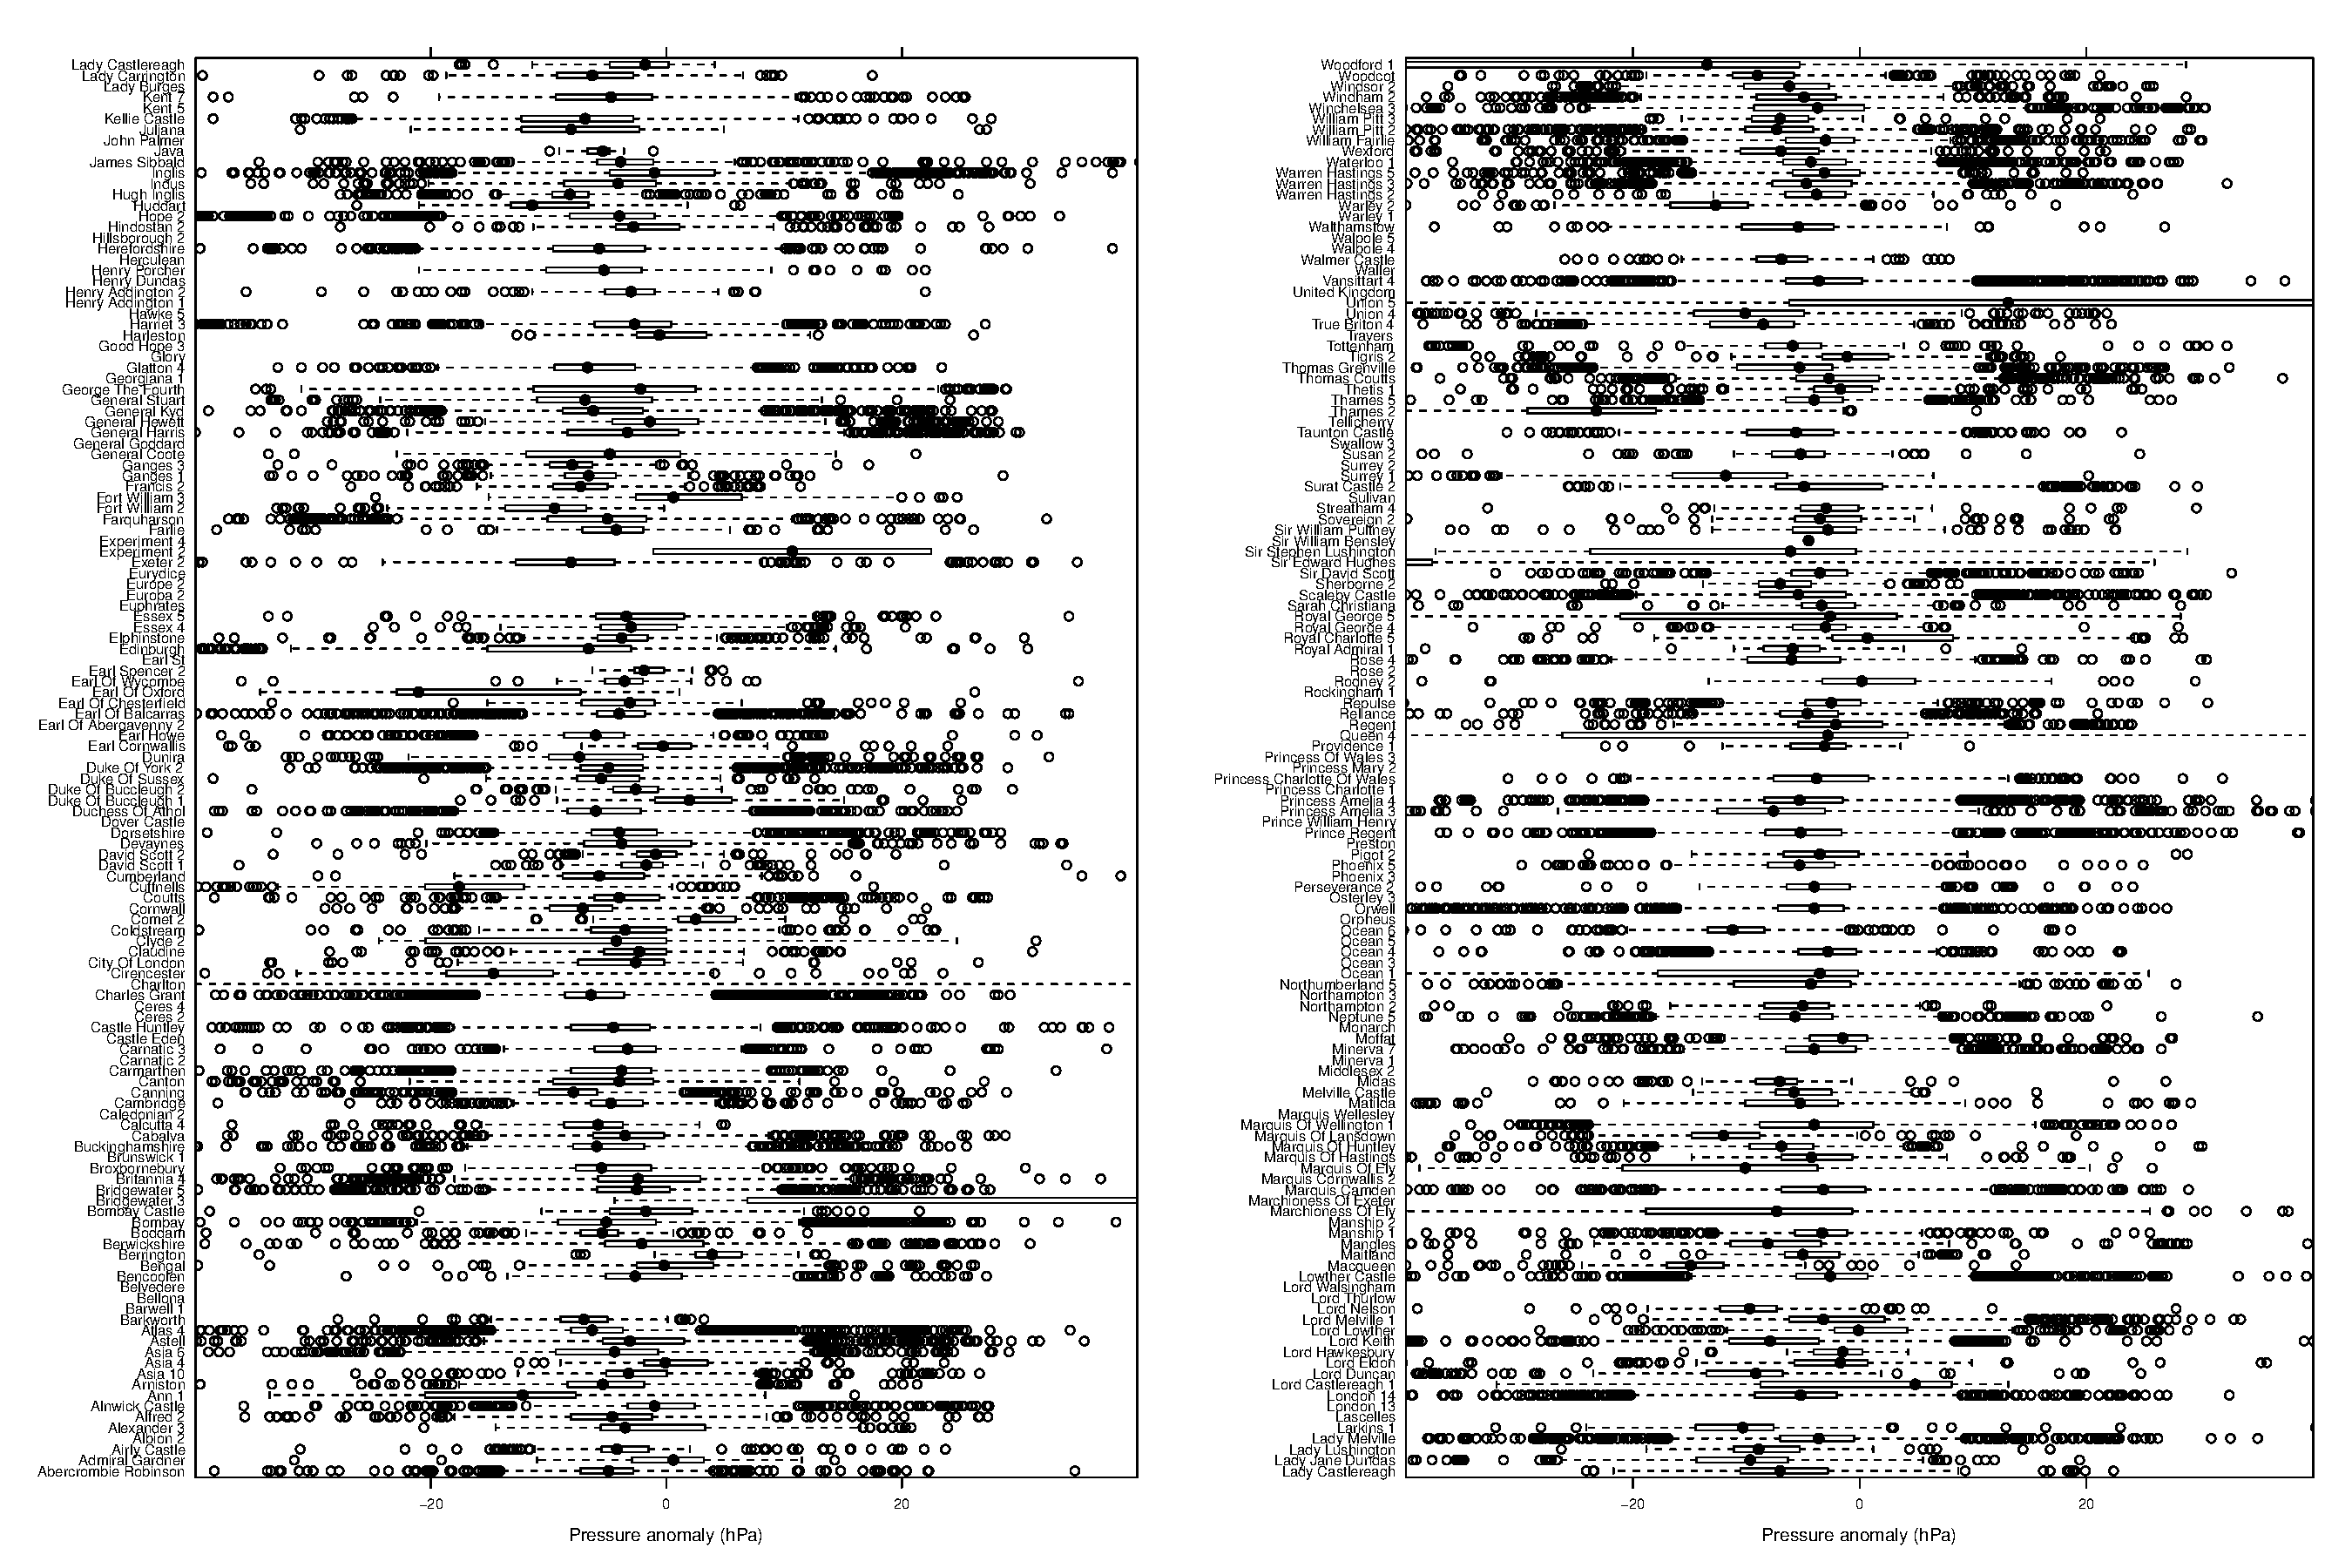
\includegraphics[angle=90, width=1.0\textwidth]{../anomaly_ts/pre_anom_bwplot_byShip}
\caption{Between-ship variability of barometer pressure anomalies (observation minus HadSLP2 climatology). Box-and-whisker plot with the anomalies aggregated by ship. [Much lower quality data than the temperatures, why?].}
\label{pre_anom_bwplot_byShip}
\end{center}
\end{figure}

\clearpage

\begin{figure}
\begin{center}
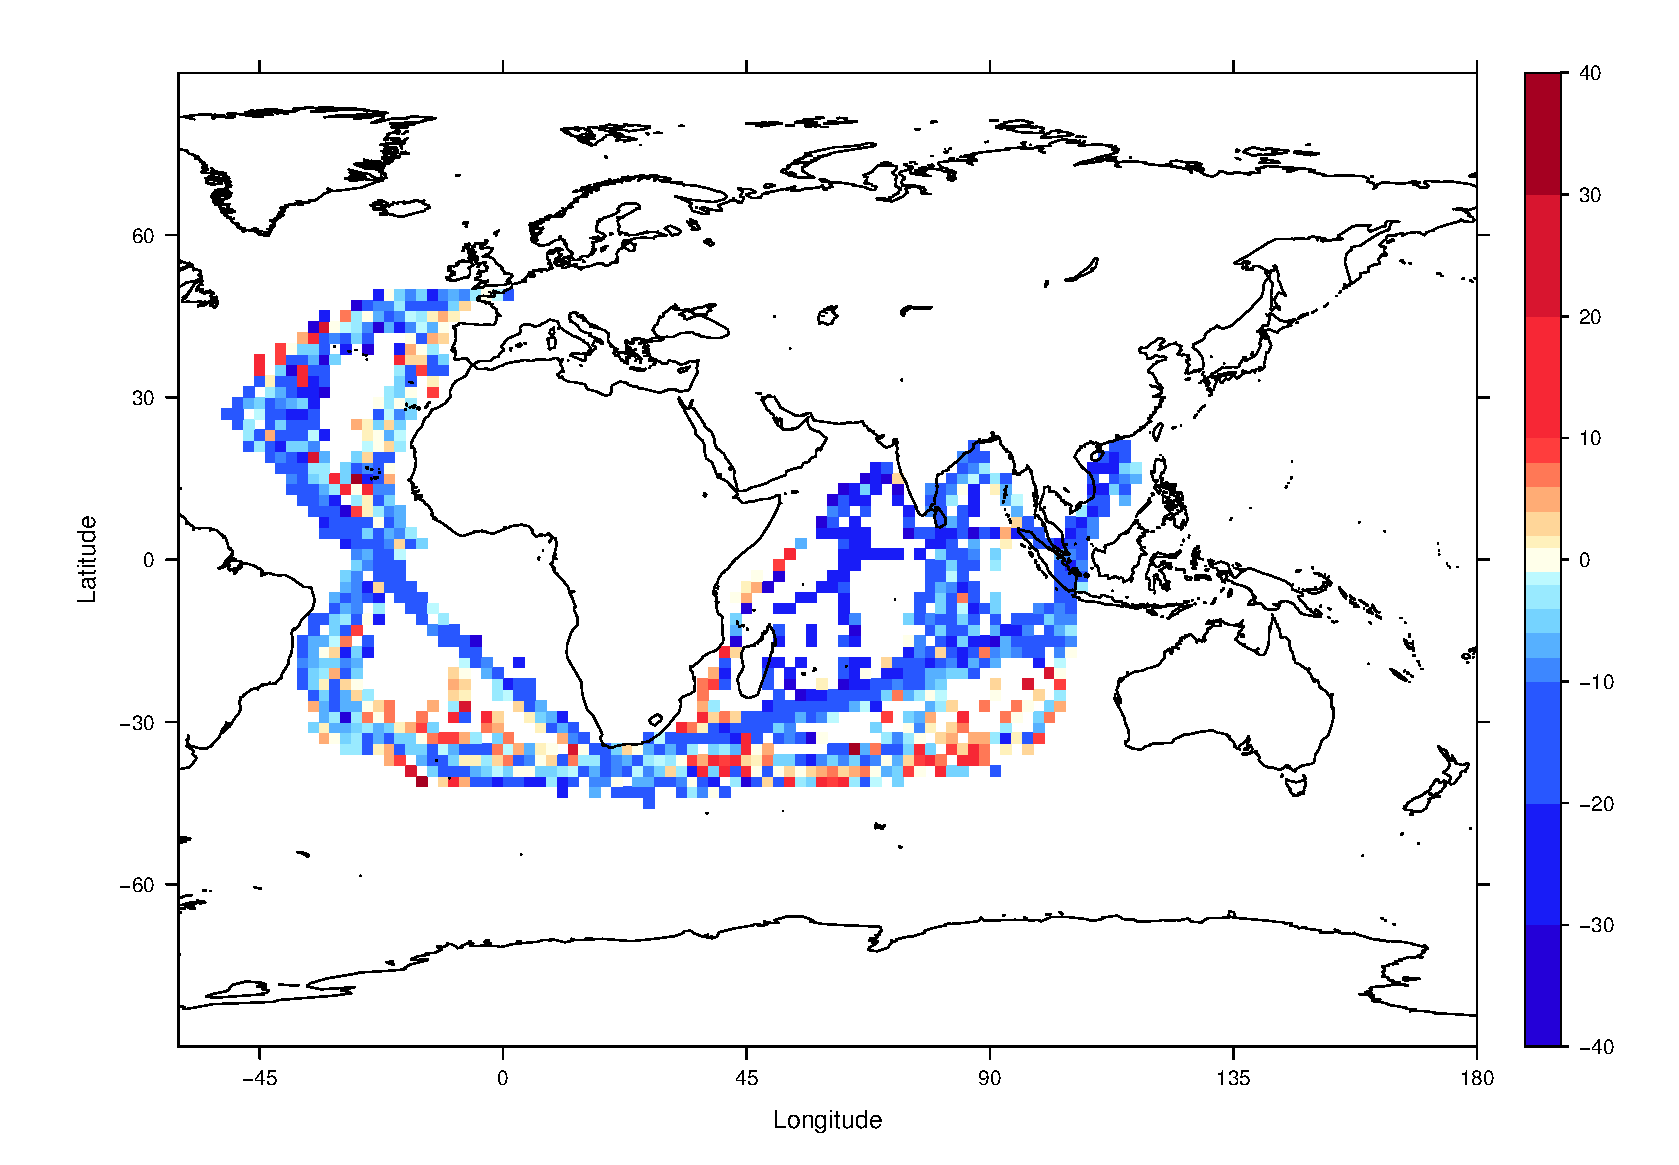
\includegraphics[angle=0, width=1.0\textwidth]{../sympiesometer/pre_anomaly_map}
\caption{Mean sympiesometer pressure anomaly (observation minus HadSLP2 climatology) in each $2^\circ$ by $2^\circ$ square. [Not much sympiesometer data, but it's even lower than the barometer pressures. I haven't applied any corrections to the sympiesiometer pressures - maybe I should?]}
\label{sym_pressure_anomaly}
\end{center}
\end{figure}

\begin{figure}
\begin{center}
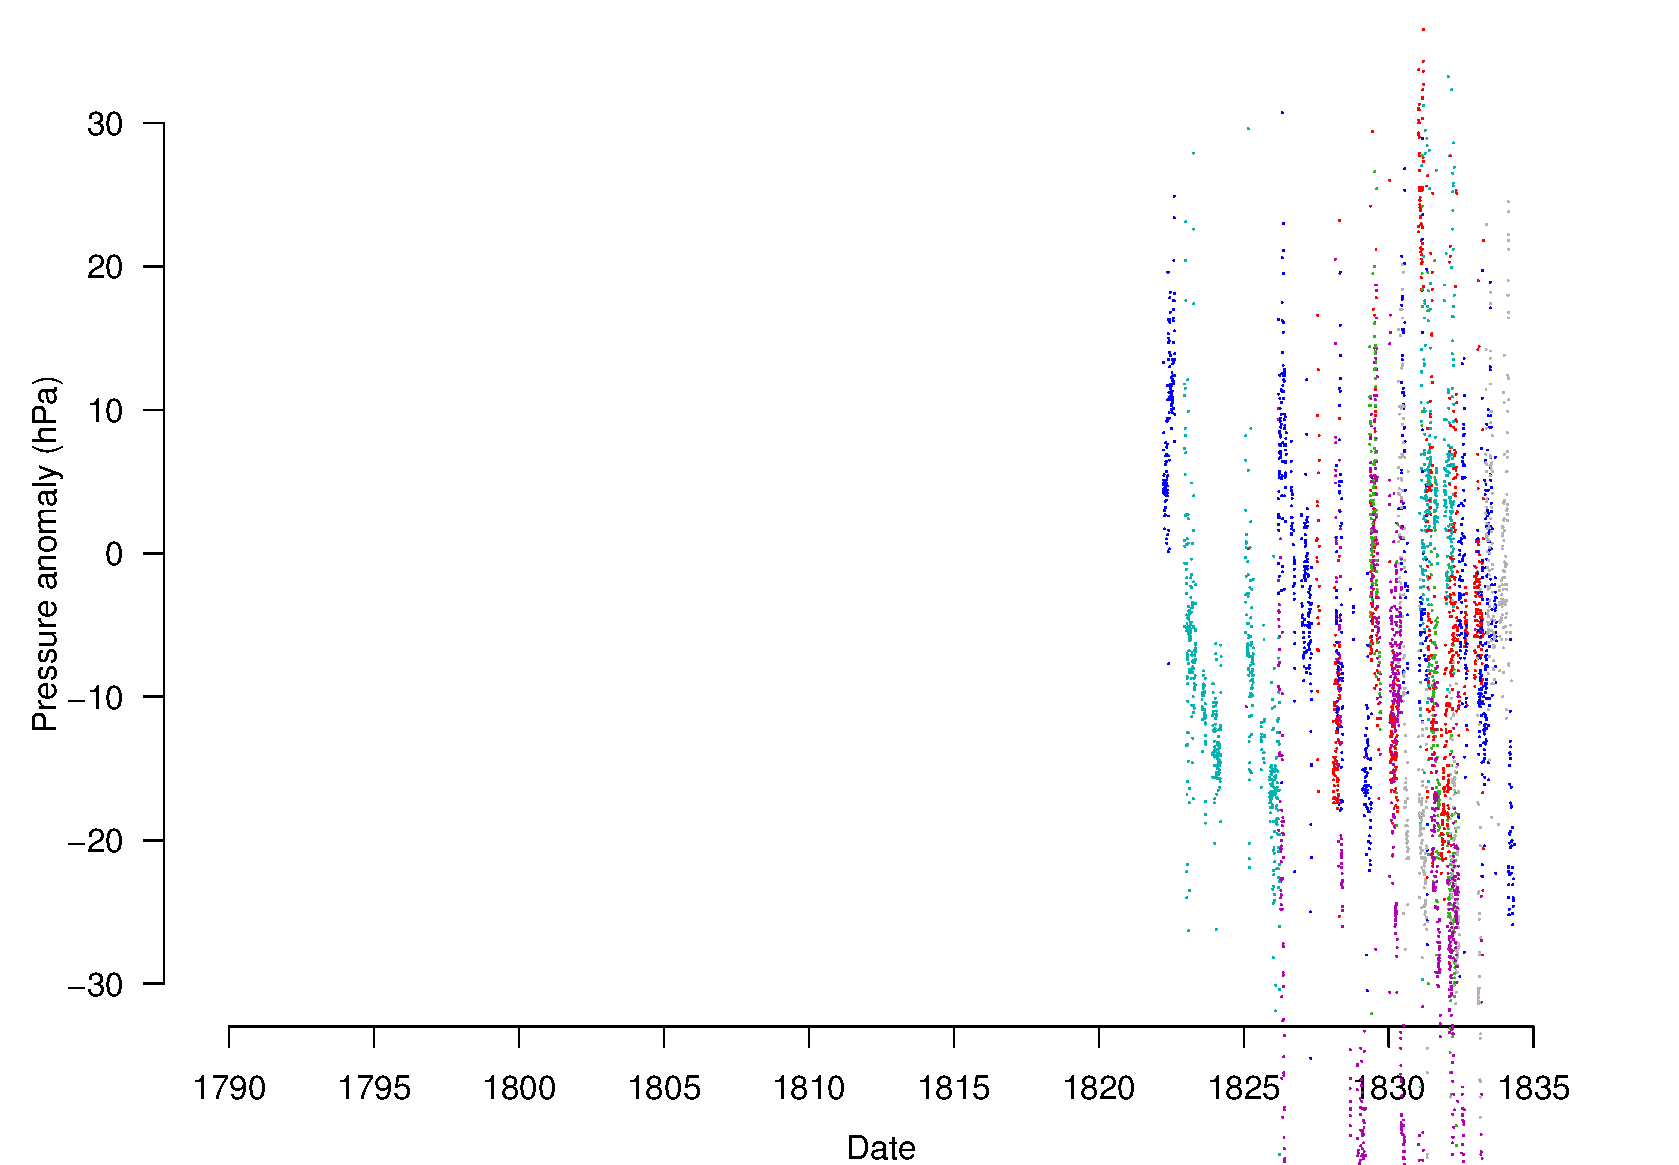
\includegraphics[angle=0, width=1.0\textwidth]{../sympiesometer/sym_anom_ts}
\caption{Time-series of sympiesometer pressure anomalies (observation minus HadSLP2 climatology). Each point is one measurement, the different colours are different ships. [All the data are from late in the period - sympiesometer was patented in 1818. Big inter-ship biases.] The really curious point is that the low bias is consistently bigger for the return voyage (India to England) than the outward voyage. }
\label{sym_pre_anom_ts}
\end{center}
\end{figure}

\begin{figure}
\begin{center}
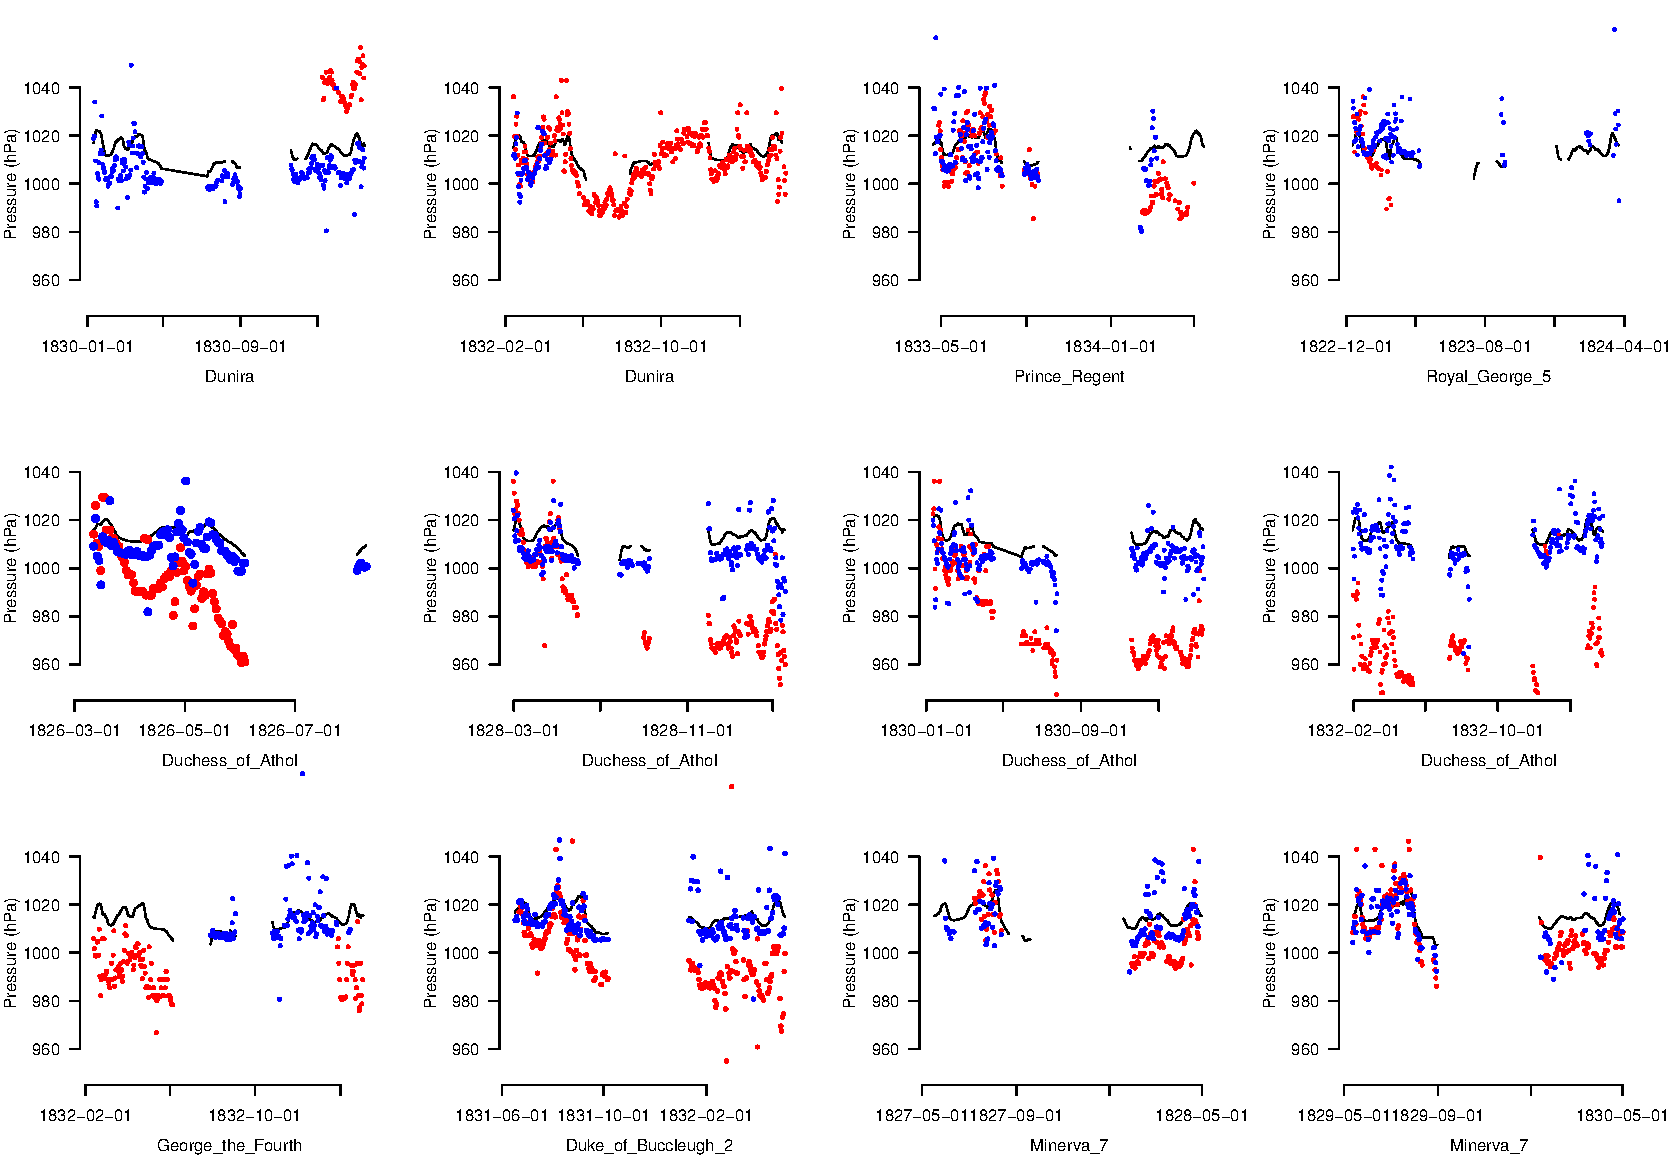
\includegraphics[angle=0, width=1.0\textwidth]{../sympiesometer/sym_v_normal_ts}
\caption{Time series of Barometric pressure (blue dots) Sympiesometer pressure (red dots), and HadSLP2 pressure normals (black lines), for voyages with sympiesometer data. [Big drifts in the sympiesometer pressures for three of the voyages - expected?]}
\label{sym_v_normal_ts}
\end{center}
\end{figure}

\begin{figure}
\begin{center}
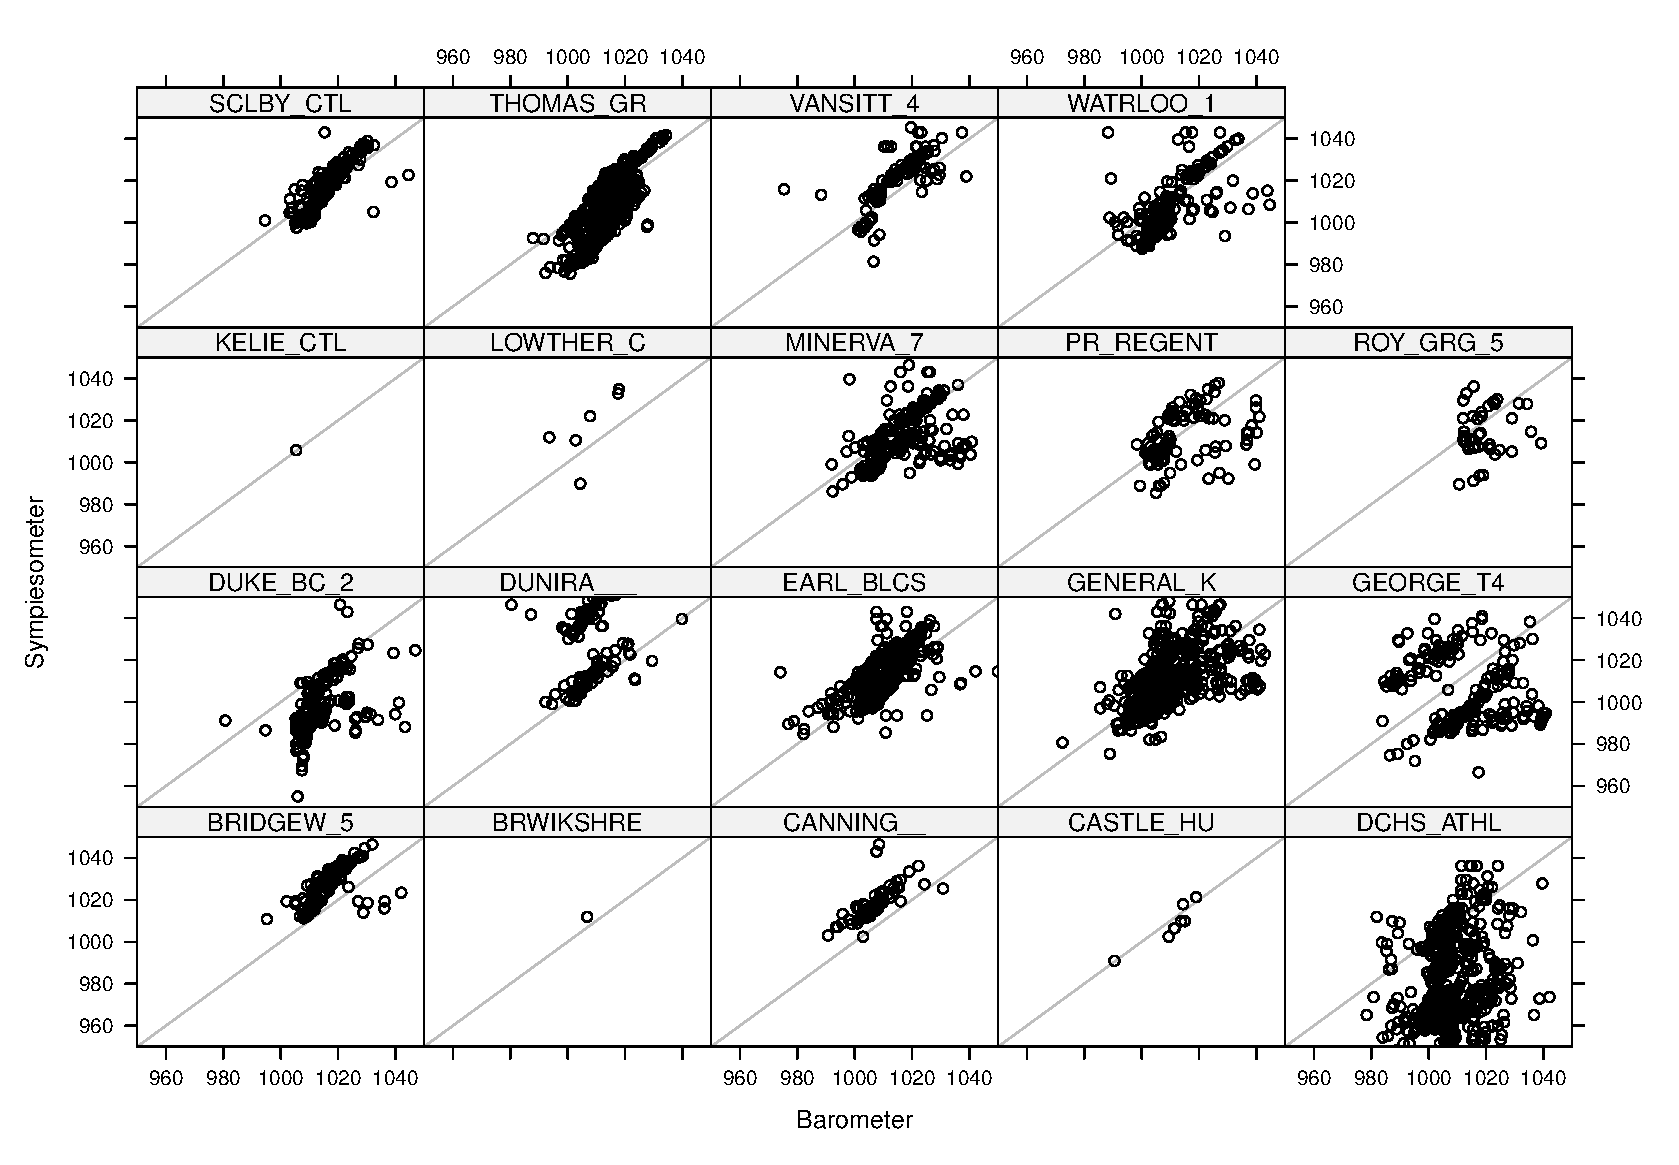
\includegraphics[angle=0, width=1.0\textwidth]{../sympiesometer/sym_v_pre}
\caption{Scatter plot of sympiesiometer pressure anomalies against barometer pressure where both are available. [As well as the bias, the sympiesiometers seem to have systematically more variation than the barometers - there is also a surprisingly large scatter. It's hard to see why the sympiesometer was popular as it seems much more prone to both drift and noise than the marine barometer.]}
\label{sym_v_pre}
\end{center}
\end{figure}

\clearpage

\begin{figure}
\begin{center}
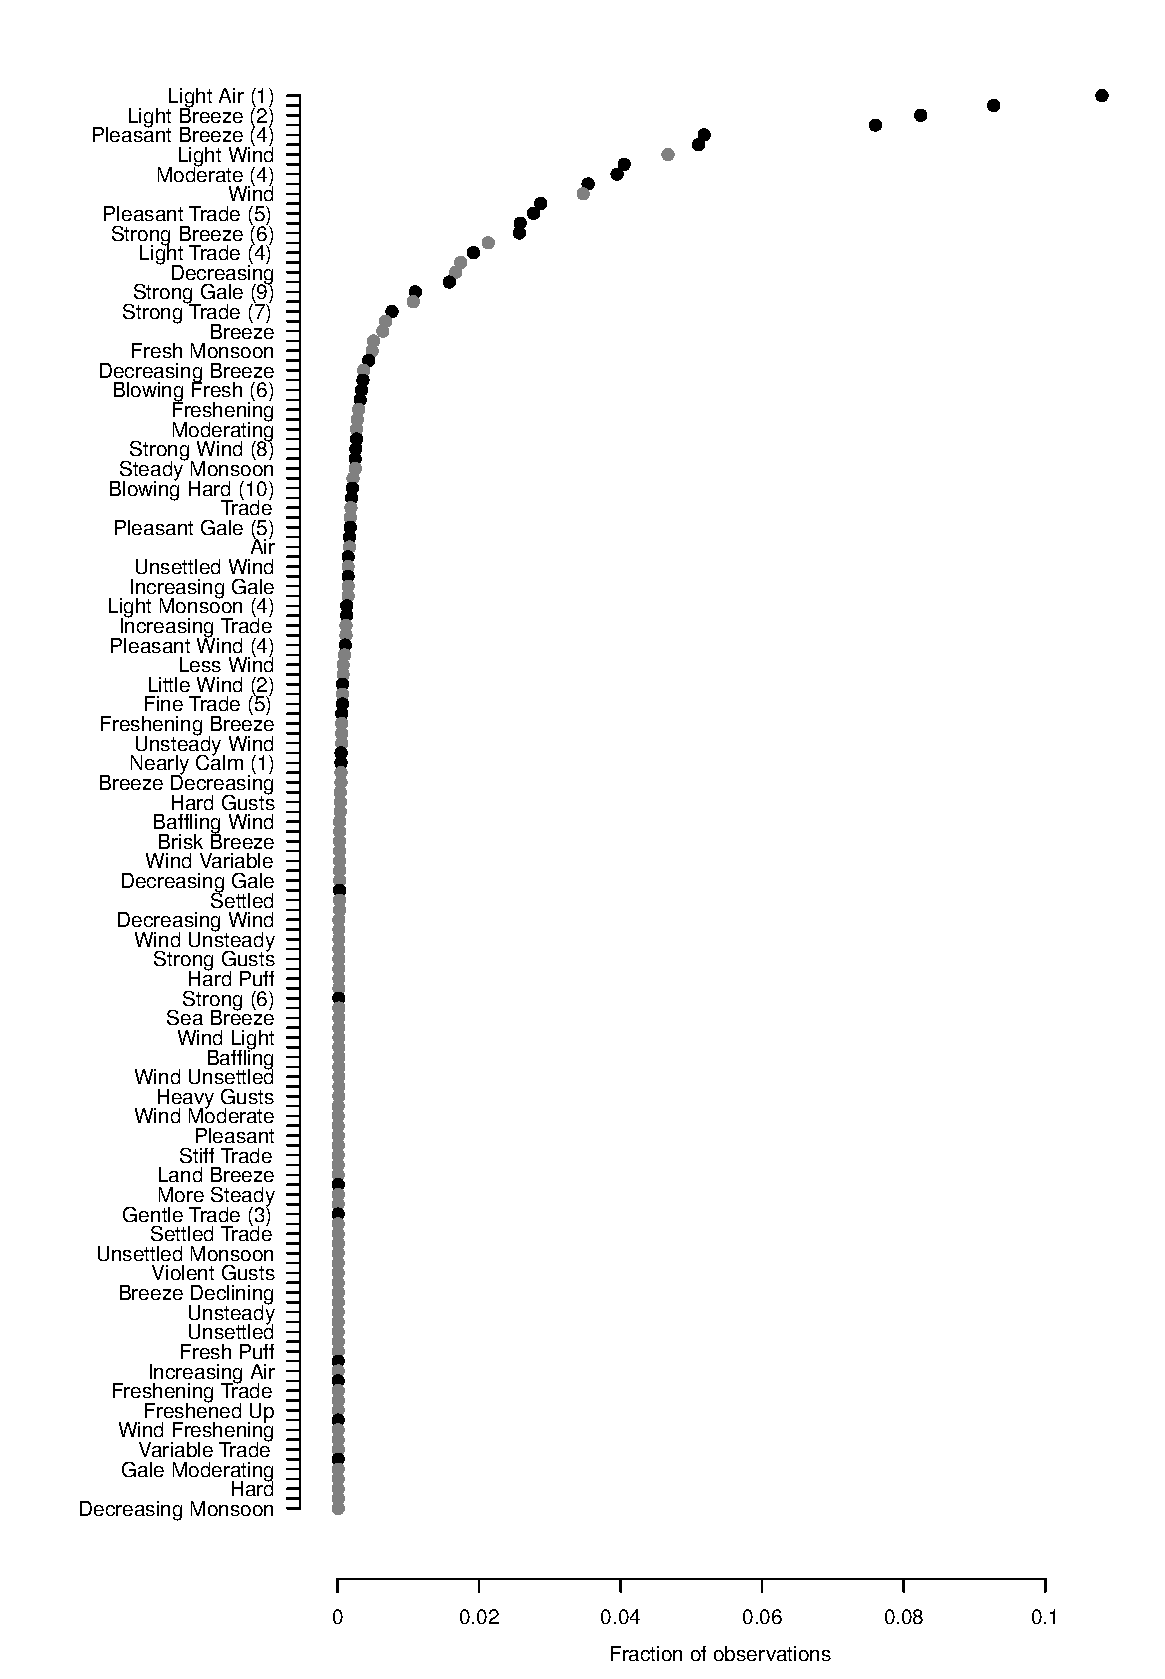
\includegraphics[angle=0, width=1.0\textwidth]{../winds/term_frequencies}
\caption{There are no instrumental observations for wind force, instead we are digitising up to two words describing the wind from each logbook page, and translating them to Beaufort force using the CLIWOC dictionary. This figure shows the relative frequency of the more common terms (all those that occur at least 10 times). Translatable terms are marked by black dots (and have the equivalent Beaufort force included in the label), terms not in the CLIWOC dictionary are marked by grey dots. [Encouraging - most records are translatable, but little obvious scope for improvement - not many frequent terms we could reasonably hope to translate. We only get wind-force terms from about half the log pages.]}
\label{wind terms}
\end{center}
\end{figure}

\begin{figure}
\begin{center}
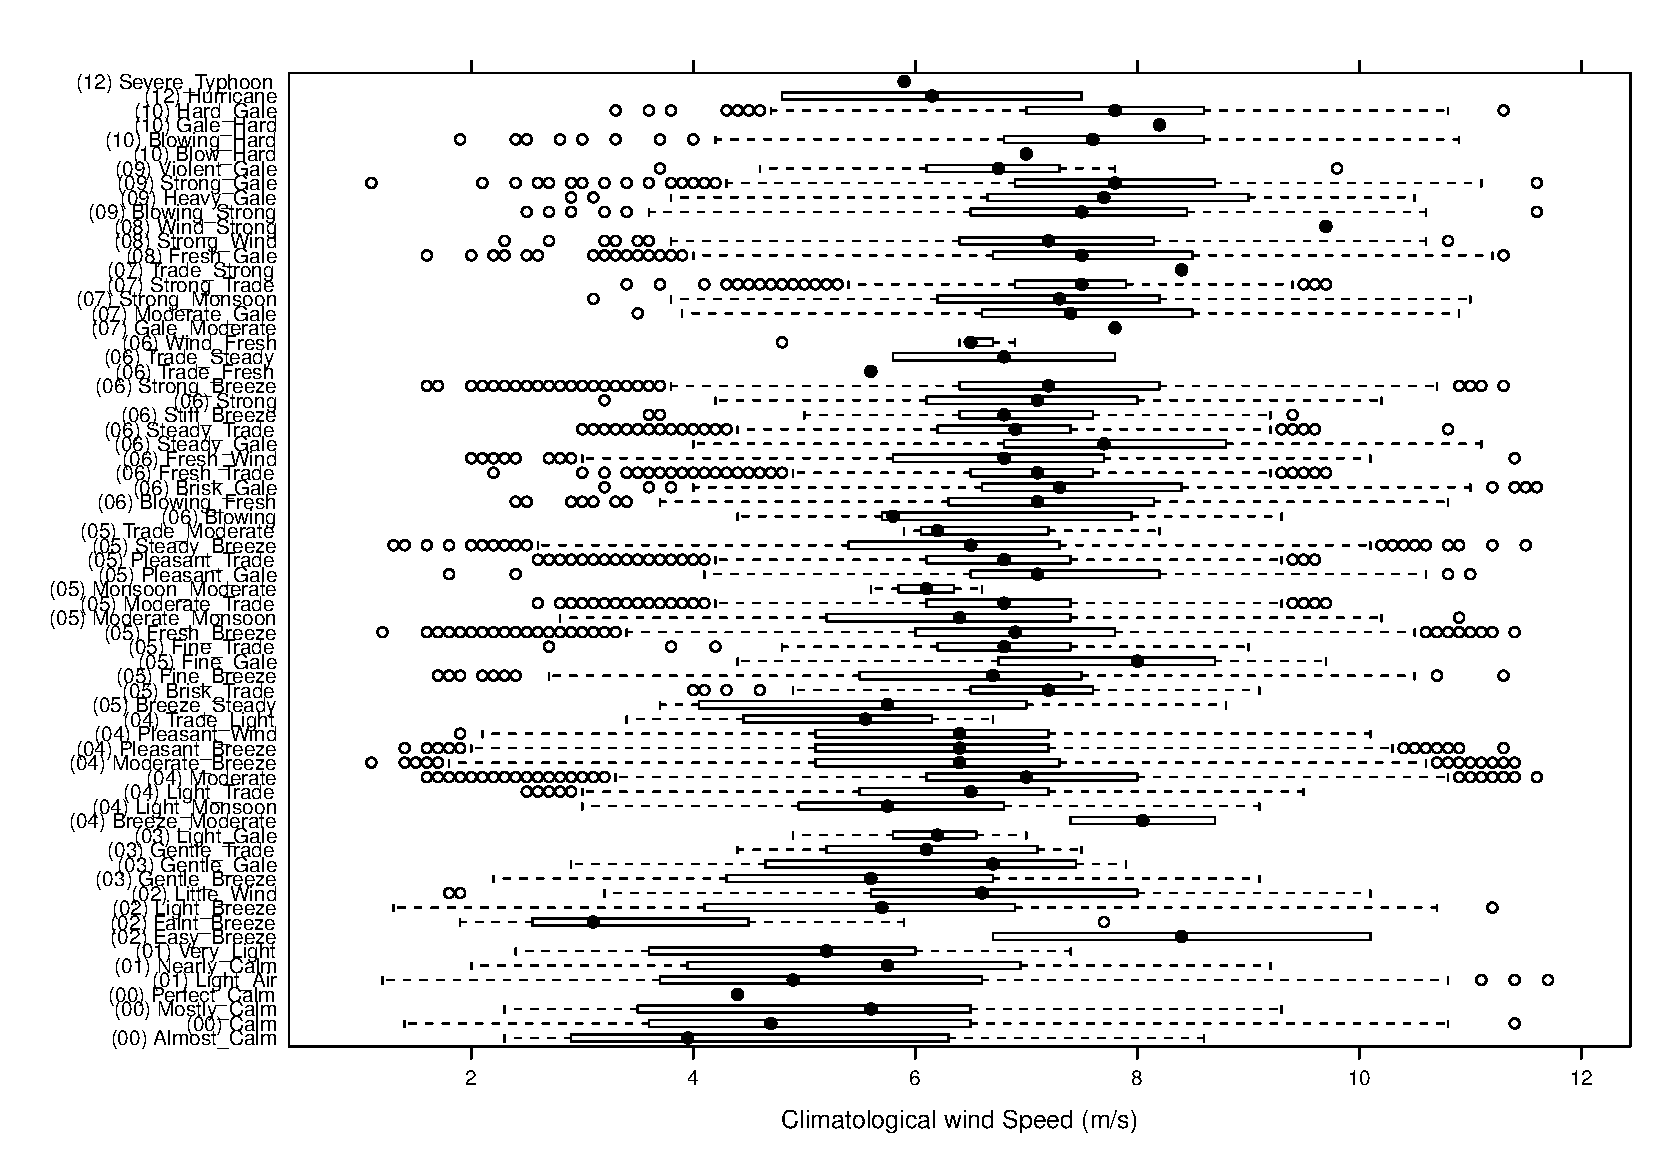
\includegraphics[angle=0, width=1.0\textwidth]{../winds/climate_v_descriptor}
\caption{Climatological wind speeds for the observations aggregated by the wind-force terms. Only those wind-force terms in the CLIWOC dictionary are included. The climatological winds are from ERA-40 at 10m height. [I'm not sure what this tells us. I was looking for indications of the reliability of the CLIWOC dictionary for the EIC obs., but I don't think this helps much - the climatological variation is too small a fraction of the total variability in wind speed. Need to compare with the ERA instantaneous winds, but that's a lot of work.]}
\label{climate_v_descriptor}
\end{center}
\end{figure}

\begin{figure}
\begin{center}
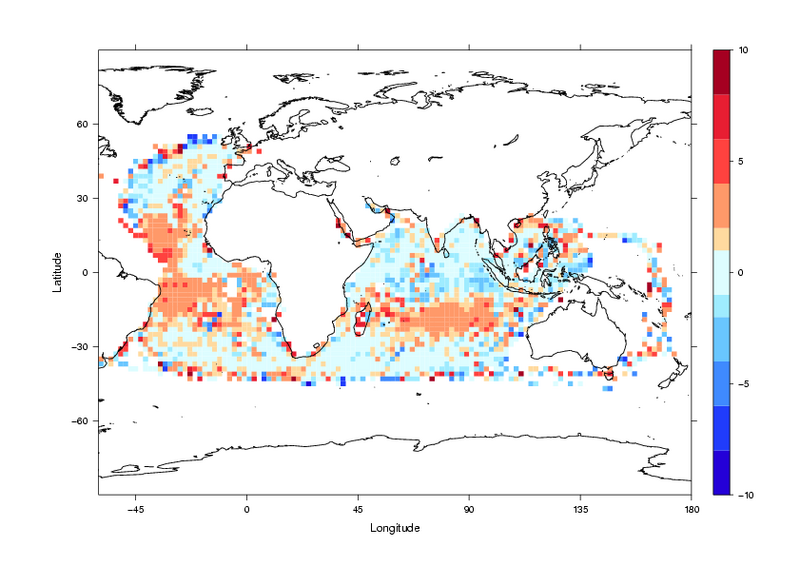
\includegraphics[angle=0, width=1.0\textwidth]{../anomaly_map/ws_anomaly}
\caption{Truncated mean wind speed anomaly ($ms^{-1}$: observation minus ERA-40 10m climatology) in each $2^\circ$ by $2^\circ$ square. [Stronger trade winds? or a bias? - could check by looking at ship speed. Need to be careful, as the observations are not random samples: stronger wind $\Rightarrow$ faster ships $\Rightarrow$ fewer observations; so I was expecting a low bias.] }
\label{ws_anomaly}
\end{center}
\end{figure}

\begin{figure}
\begin{center}
\includegraphics[angle=0, width=1.0\textwidth]{../anomaly_ts/ws_anom_ts}
\caption{Time-series of wind-speed anomalies (observation minus ERA-40 10m climatology). Each point is one measurement, the different colours are different ships (though there are more ships than available colours). [No alarming inconsistencies.]}
\label{ws_anom_ts}
\end{center}
\end{figure}

\begin{figure}
\begin{center}
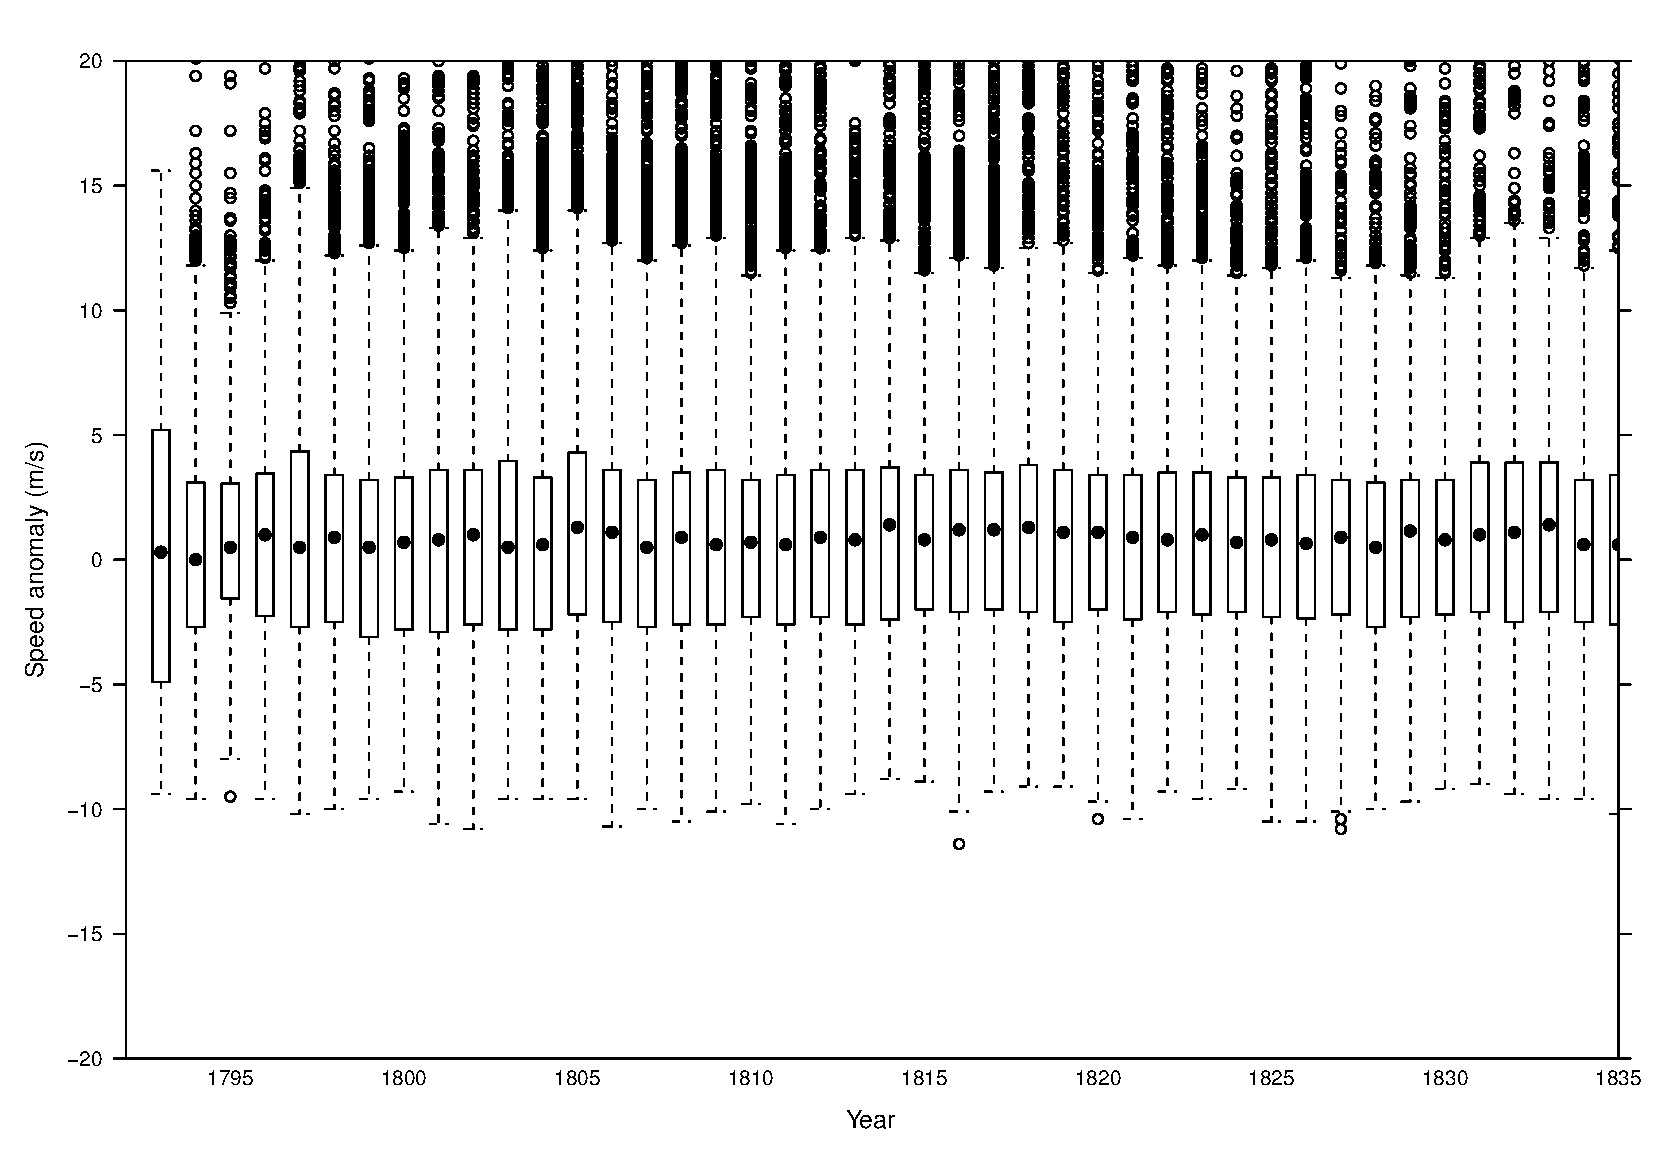
\includegraphics[angle=0, width=1.0\textwidth]{../anomaly_ts/ws_anom_bwplot}
\caption{Time-series of wind-speed anomalies (observation minus ERA-40 10m climatology). Box-and-whisker plot with the anomalies aggregated by calendar year. [Observed winds have a long tail to high speeds, hence the asymmetry in anomalies.]}
\label{ws_anom_bwplot}
\end{center}
\end{figure}

\begin{figure}
\begin{center}
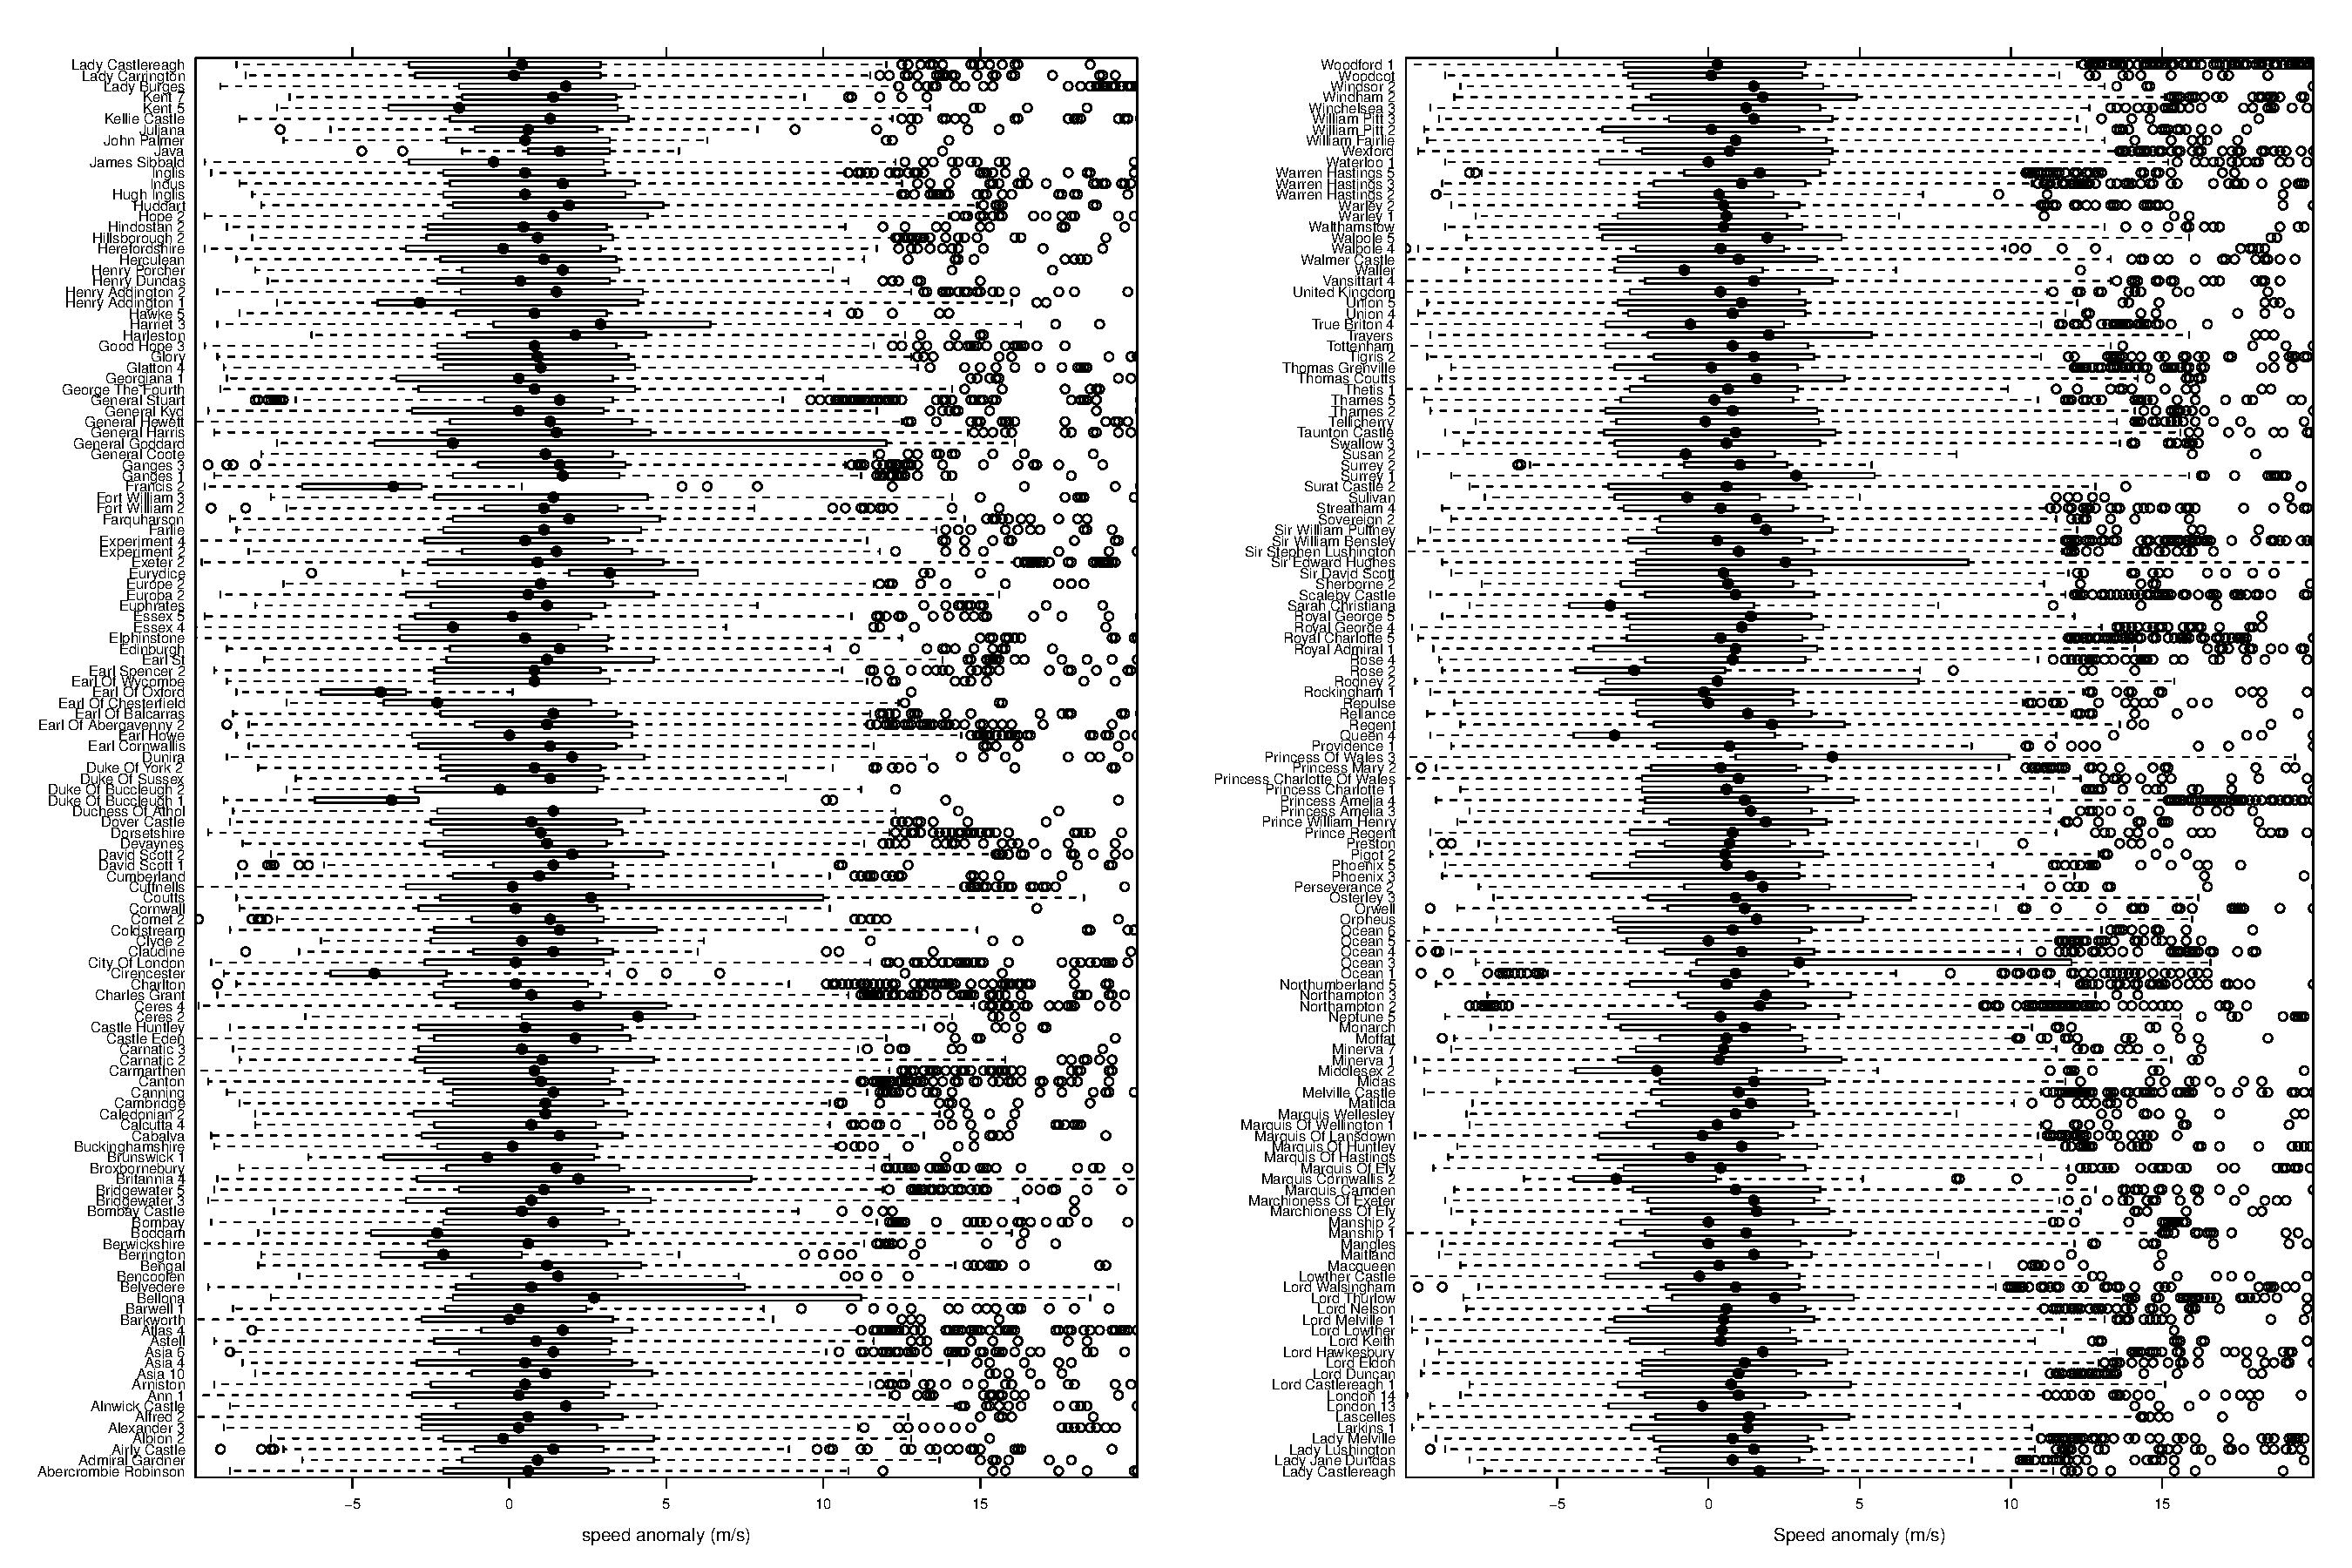
\includegraphics[angle=90, width=1.0\textwidth]{../anomaly_ts/ws_anom_bwplot_byShip}
\caption{Between-ship variability of wind-speed anomalies (observation minus ERA-40 10m climatology). Box-and-whisker plot with the anomalies aggregated by ship. [Large interquartile ranges tend to be associated with ships with few observations, so maybe not a statistically significant difference - check.]}
\label{ws_anom_bwplot_byShip}
\end{center}
\end{figure}



\end{document}
